\documentclass{beamer}
\usetheme{CambridgeUS}
% \usetheme[secheader]{Boadilla}
 
\usepackage{fontspec}
\usepackage{amsmath,amsfonts,amssymb}
\usepackage{booktabs}
\usepackage{caption}
\usepackage{subcaption}
\usepackage{graphicx}
\usepackage{float}
\usepackage{fancyhdr}
\usepackage{bm}
\usepackage{multirow}
\usepackage{multirow}
\usepackage{tabularx}
\usepackage[final]{pdfpages}
\usepackage{pdfpages}
\setsansfont{STFangsong} % font name is case-sensitive
 
\begin{document}
\title{$L_1$因子分析及其在宏观经济中的应用} 
\author{答辩人:蒯强\ \ 导师:孔新兵 教授}
\institute[]{南京审计大学统计与数学学院} % 设置学院机构
\logo{
\includegraphics[width=1.2cm,height=1.2cm]{pics/avatar.jpeg}}

\frame{\titlepage}

\section{选题背景}

\begin{frame}{宏观经济和政府调控}

  \begin{itemize}
\item
政府是指导和调控经济运行的主体。国民经济的发展和政府的指导
和调控紧密相关。

\item
政府部门需要时刻把握国民经济的方方面面,要研究这些经济变量
发生变化的原因以及各种经济变量
之间的作用关系。

\item
只有这样,政府才能发现经济中存在的问题,并且给出针对性的指
导和调控手段。
  \end{itemize}
\end{frame}

\begin{frame}{把控宏观经济数据}
  \begin{itemize}
    \item
    政府需要时刻把控宏观经济指标的当前水平。
  \end{itemize}
\begin{figure}[H]
  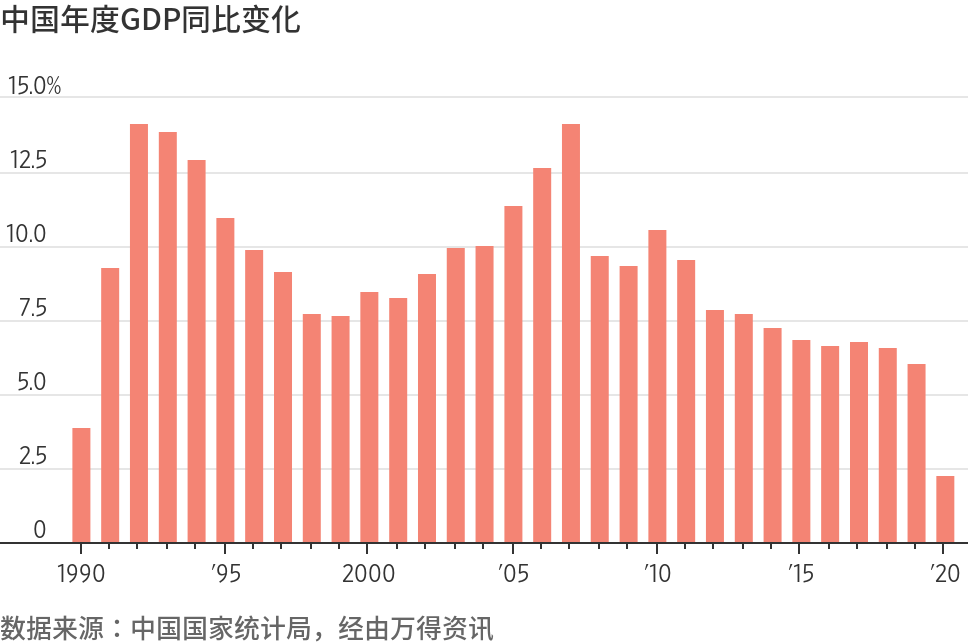
\includegraphics[width=5cm]{pics/gdp.png}
  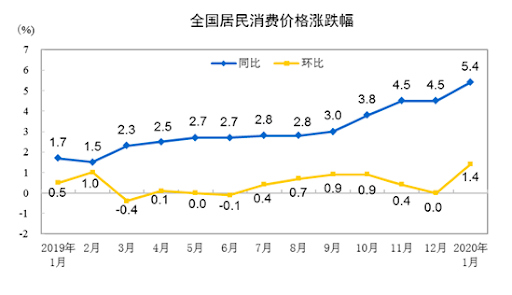
\includegraphics[width=5cm]{pics/price.png}
\end{figure}
\end{frame}

\begin{frame}{宏观经济现状分析}
  \begin{itemize}
    \item
    通过对当前宏观经济指标数据的综合分析,观察当前宏观经济
    的运行状况,便于行使见机行事的宏观经济政策。
  \end{itemize}
\begin{figure}[H]
  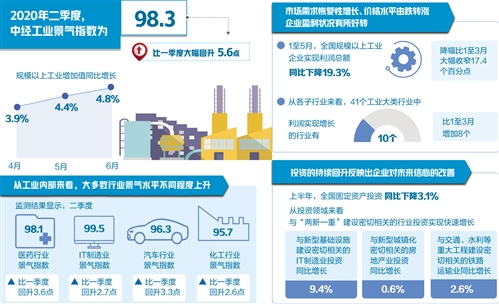
\includegraphics[width=8cm]{pics/macro-demo.jpeg}
\end{figure}
\end{frame}

\begin{frame}{宏观经济预测}
  \begin{itemize}
    \item
    政府和研究机构常常对重要经济指标做出预测
  \end{itemize}
\begin{figure}[H]
  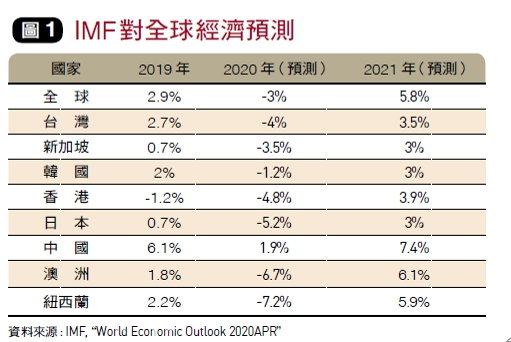
\includegraphics[width=8cm]{pics/predict-demo.jpeg}
\end{figure}
\end{frame}

\begin{frame}{宏观经济预测}

\begin{figure}[H]
  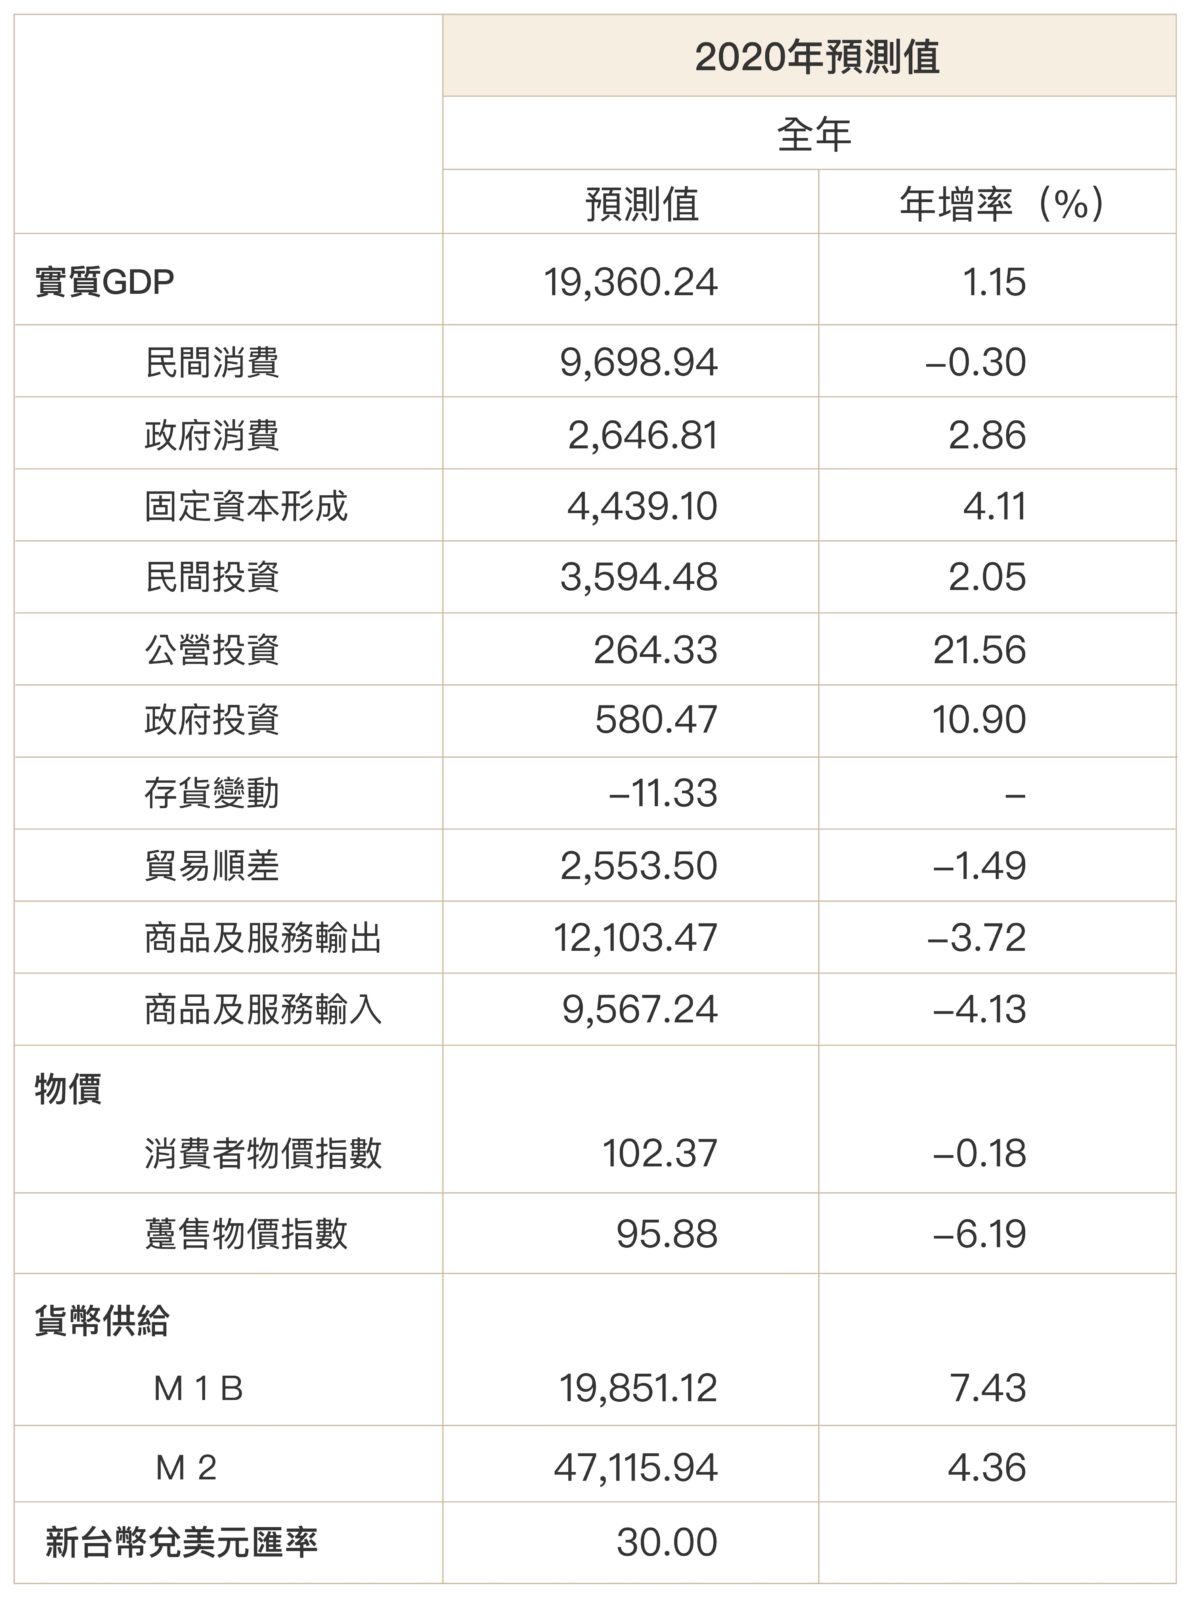
\includegraphics[width=6cm]{pics/predict-demo2.jpeg}
\end{figure}

\end{frame}


\begin{frame}{高维宏观经济数据}
  \begin{itemize}
    \item
    宏观经济指标往往是高维的,难以采用传统模型进行分析。
  \end{itemize}
  \begin{figure}[H]
    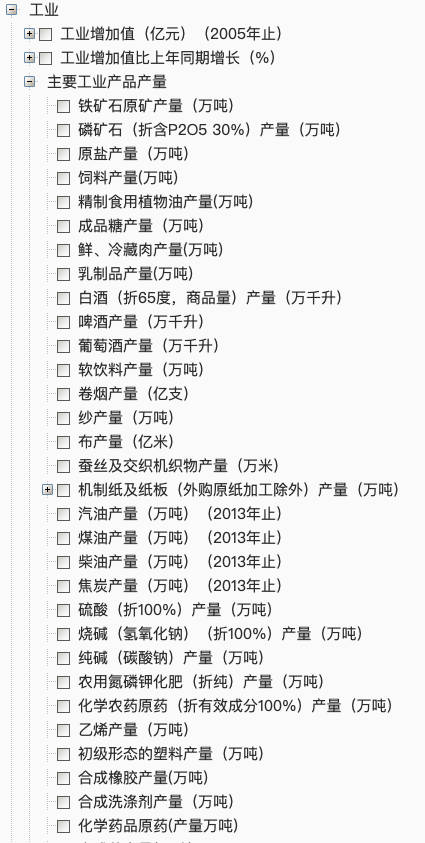
\includegraphics[width=4cm]{pics/var1.png}
    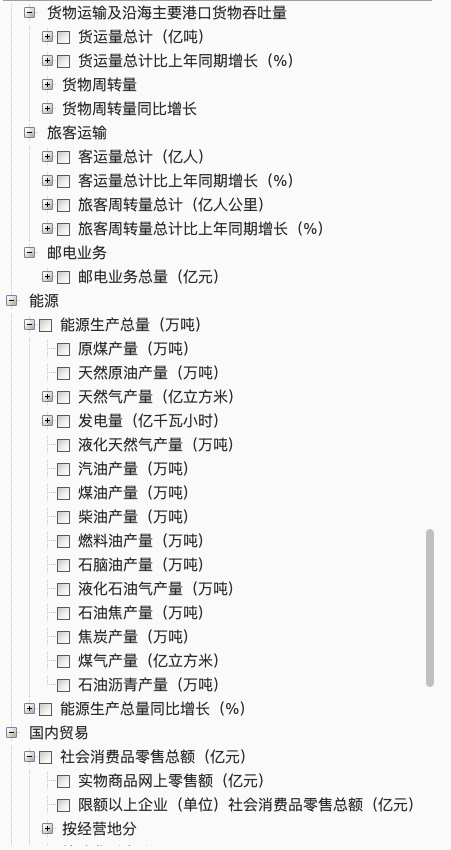
\includegraphics[width=4cm]{pics/var2.png}
  \end{figure}
  
\end{frame}

\section{扩散指数模型}
\begin{frame}{因子分析是分析高维宏观经济数据的常用手段}

\begin{figure}[H]
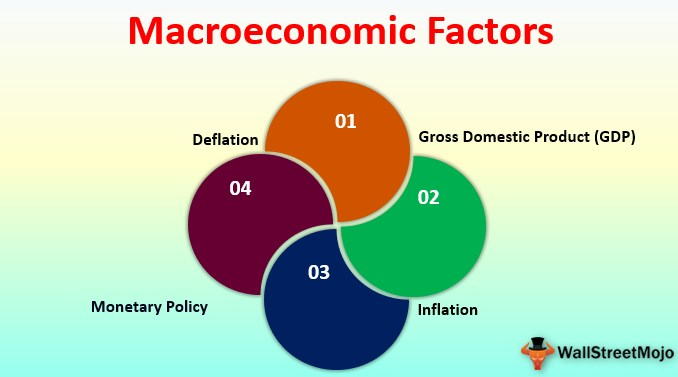
\includegraphics[width=8cm]{pics/macroeco-demo.jpeg}
\end{figure}

\end{frame}

\begin{frame}{扩散指数模型进行宏观经济预测}
        \ \ \ \ 令$y_t$为待预测经济变量$y$在时间$t$的水平,$\bm{X}_t$为$p$维随机向量,
        假设$(X_t,y_t)$服从近似因子模型并且$\bm{X}_t$和$y_t$具有相依性,若$\bm{X}_t, y_t$
        有$m$维共同因子$\bm{F}_t$,即
    \begin{equation}
        \bm{X}_t = \bm{A}\bm{F}_t + \bm{e}_t
    \end{equation}
    则可以通过式\eqref{predict-factor-model}对$y_{t+h}$进行预测,
    \begin{equation}\label{predict-factor-model}
        y_{t+h} = \bm{\beta}(L)\bm{F}_t + \bm{\alpha}(L)y_t + c + e_{t+h}
    \end{equation}
    其中滞后算子$\bm{\beta}(L)$反映了共同因子滞后项的影响,而$\bm{\alpha}(L)$
    表示$y_t$自身的滞后项的影响。
\end{frame}

\begin{frame}{扩散指数模型进行宏观经济预测}
    \begin{figure}[H]
        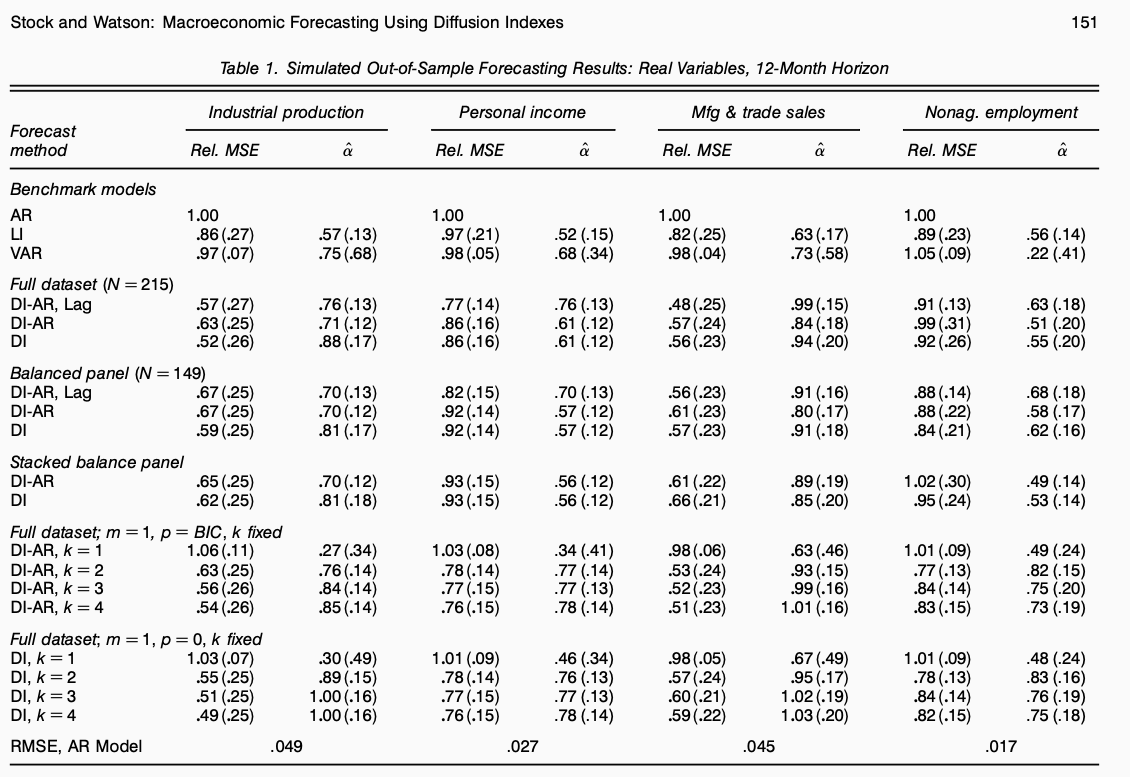
\includegraphics[width=10cm]{pics/stock.png}
        \end{figure}
\end{frame}

\begin{frame}{扩散指数模型的因子估计}
    为了得到因子序列,需要对静态因子进行估计,Stock和Watson采用
    主成分分析作为非参数估计。
    \begin{figure}[H]
        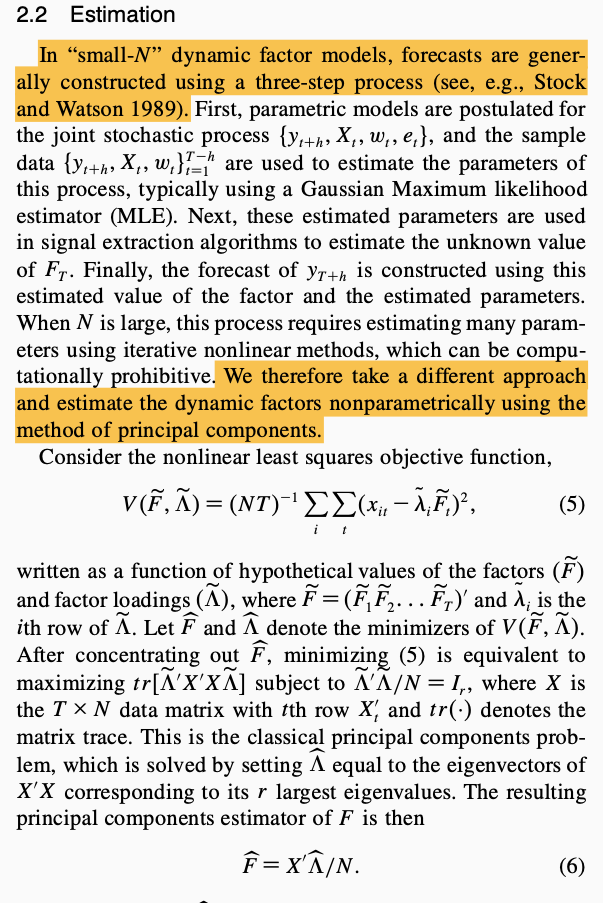
\includegraphics[width=6cm]{pics/stock-principle.png}
        \end{figure}
\end{frame}

\begin{frame}{主成分分析法}
    \begin{itemize}
        \item
        主成分分析法是常见的降维方法。
    \end{itemize}
\end{frame}

\section{$L_1$因子分析}


\begin{frame}{$L_2$主成分分析不稳健}
    \begin{itemize}
        \item
        $L_2$主成分分析对离群值不稳健。
      \end{itemize}
    \begin{figure}[H]
        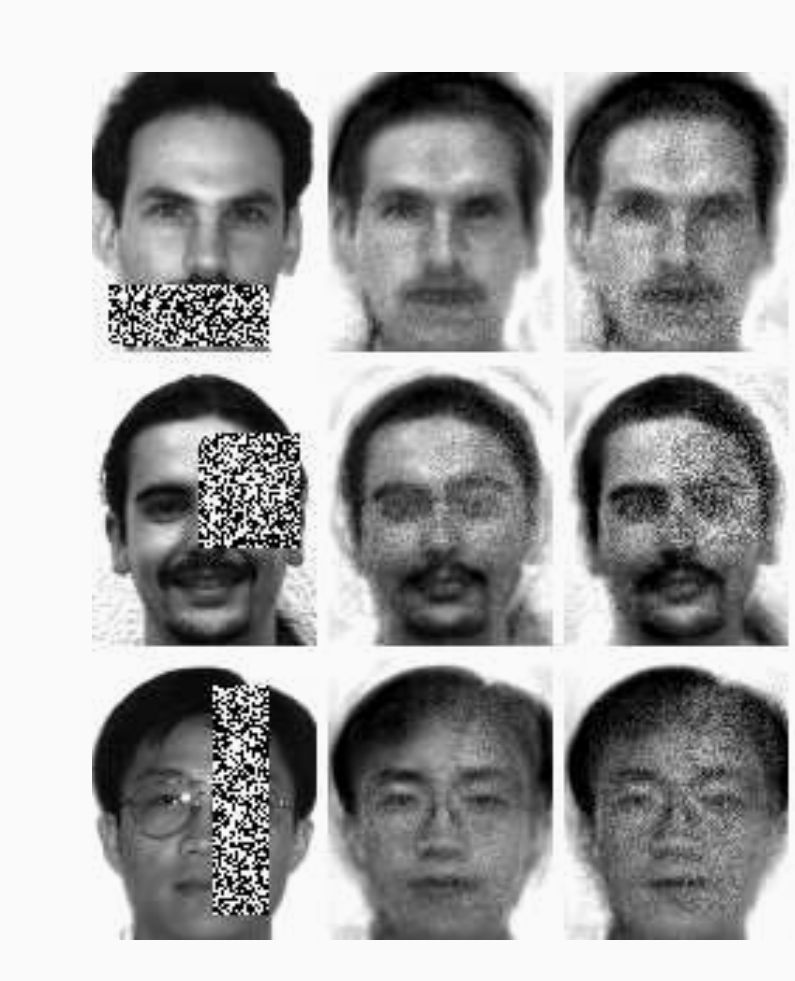
\includegraphics[width=5cm]{pics/face.png}
    \end{figure}
\end{frame}

\begin{frame}{
    $L_1$和$L_2$的稳健性对比}
    \begin{itemize}
        \item
        $L_1$范数能够提供更好的稳健性。
      \end{itemize}
    \begin{figure}[H]
        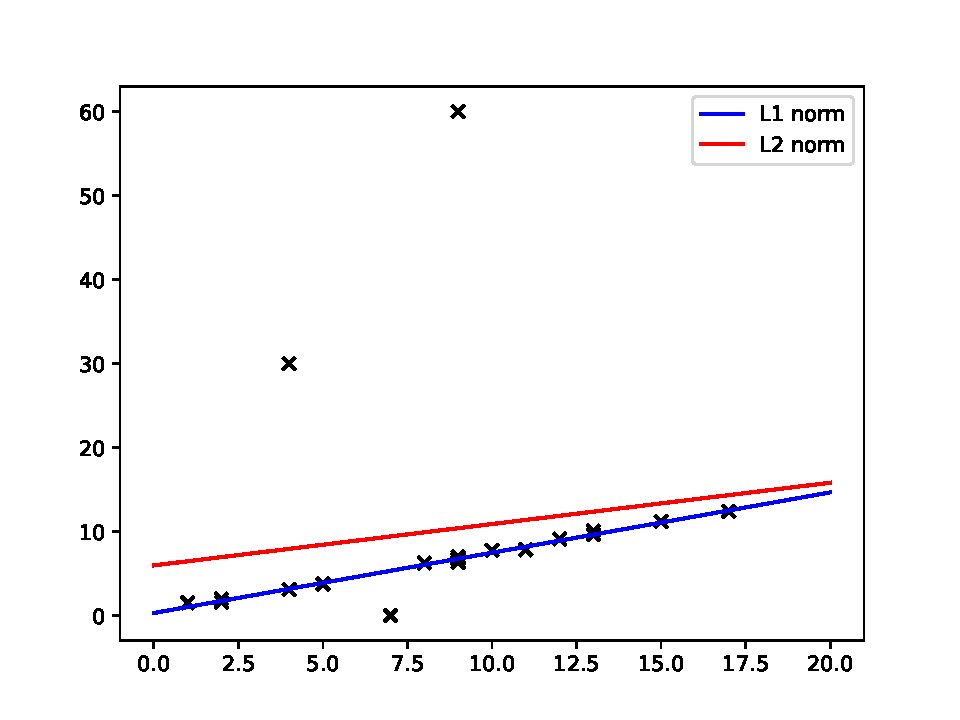
\includegraphics[width=5cm]{pics/l1-l2-diff.pdf}
        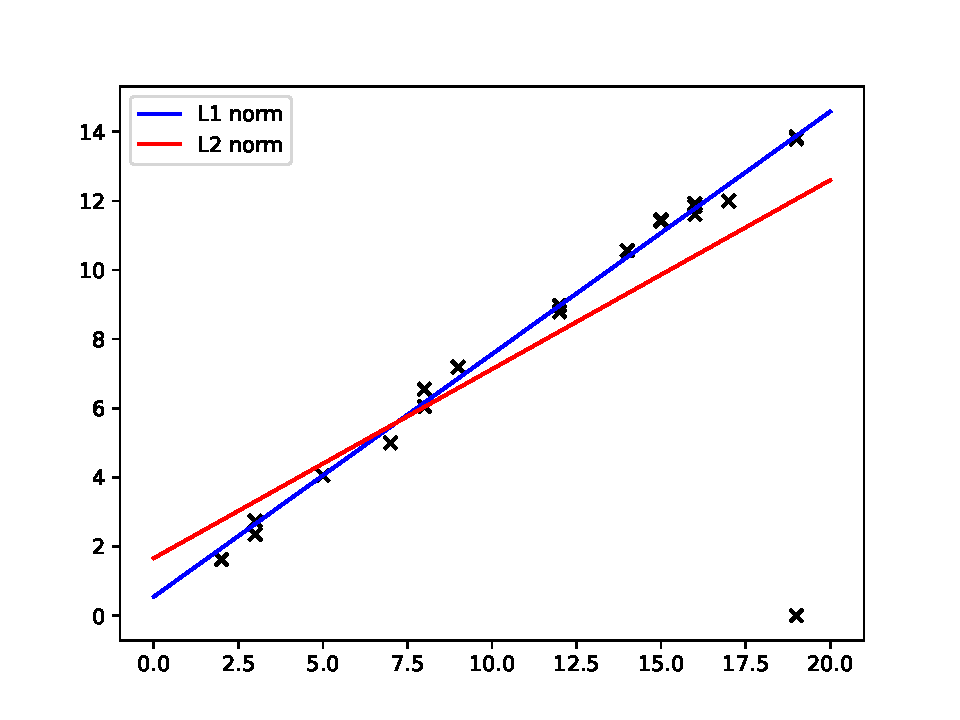
\includegraphics[width=5cm]{pics/l1-l2-diff2.pdf}
    \end{figure}
\end{frame}


\begin{frame}{$L_2$主成分分析问题描述}
    \begin{itemize}
        \item
        $L_2$主成分分析问题描述
    \end{itemize}
    \small
    \begin{equation}\label{pca-l2-p1}
        P_1: \ \hat{\bm{A}}_{p\times m}, \hat{\bm{F}}_{m\times n} = \underset{\bm{A},\bm{F}}{\operatorname{arg\ min} } 
        \|\bm{X} - \bm{A}\bm{F}\|_{L_2}
         = \underset{\bm{A}, \bm{F}}{\operatorname{arg\ min}} \sum_{i=1}^p \sum_{j=1}^m (x_{ij} - \bm a_i^T\bm f_i)^2 ,
        \end{equation}
    \tiny
        其中$\bm{X}$为$p \times n$的高维数据矩阵,$\bm{A}$的列构成了$\bm{X}$的$m$维线性子空间的基,这个子空间也称为特征空间。
        $\bm{F}$为一系数矩阵,给出了$\bm{X}$各列元素在特征空间中的坐标,根据矩阵投影理论,在给定$\bm{A}$的条件下,
        $\bm{F} = \bm{A}^T \bm{X}$。
        问题$P_1$可以解释为,需要找到一个合适的投射矩阵,使得数据在低维的投影上升回高维空间后和原矩阵各元素的误差平方和最小。
        
        对于问题$P_1$常用奇异值分解法求解。同样地我们也可考虑其对偶问题$P_2$,
    \small
        \begin{equation}\label{pca-l2-p2}
        P_2: \ \hat{\bm{A}} = \underset{\bm{A}}{\operatorname{arg\ max}} \| \bm{A}^T \bm{X}\|_{L_2}, \text{其中}\ \bm{A}^T
        \bm{A} = \bm{I}_m.
        \end{equation}
    \tiny
    问题$P_2$可以理解为,需要找到一个合适的投射矩阵,使得数据在低维空间的投影有最大的方差。在统计学上,数据的方差反映了
    数据中信息的多少,因此在特征空间中选取方差最大的方向作为主成分是很恰当的。
\end{frame}

\begin{frame}{重构误差最小化}
    \begin{figure}
        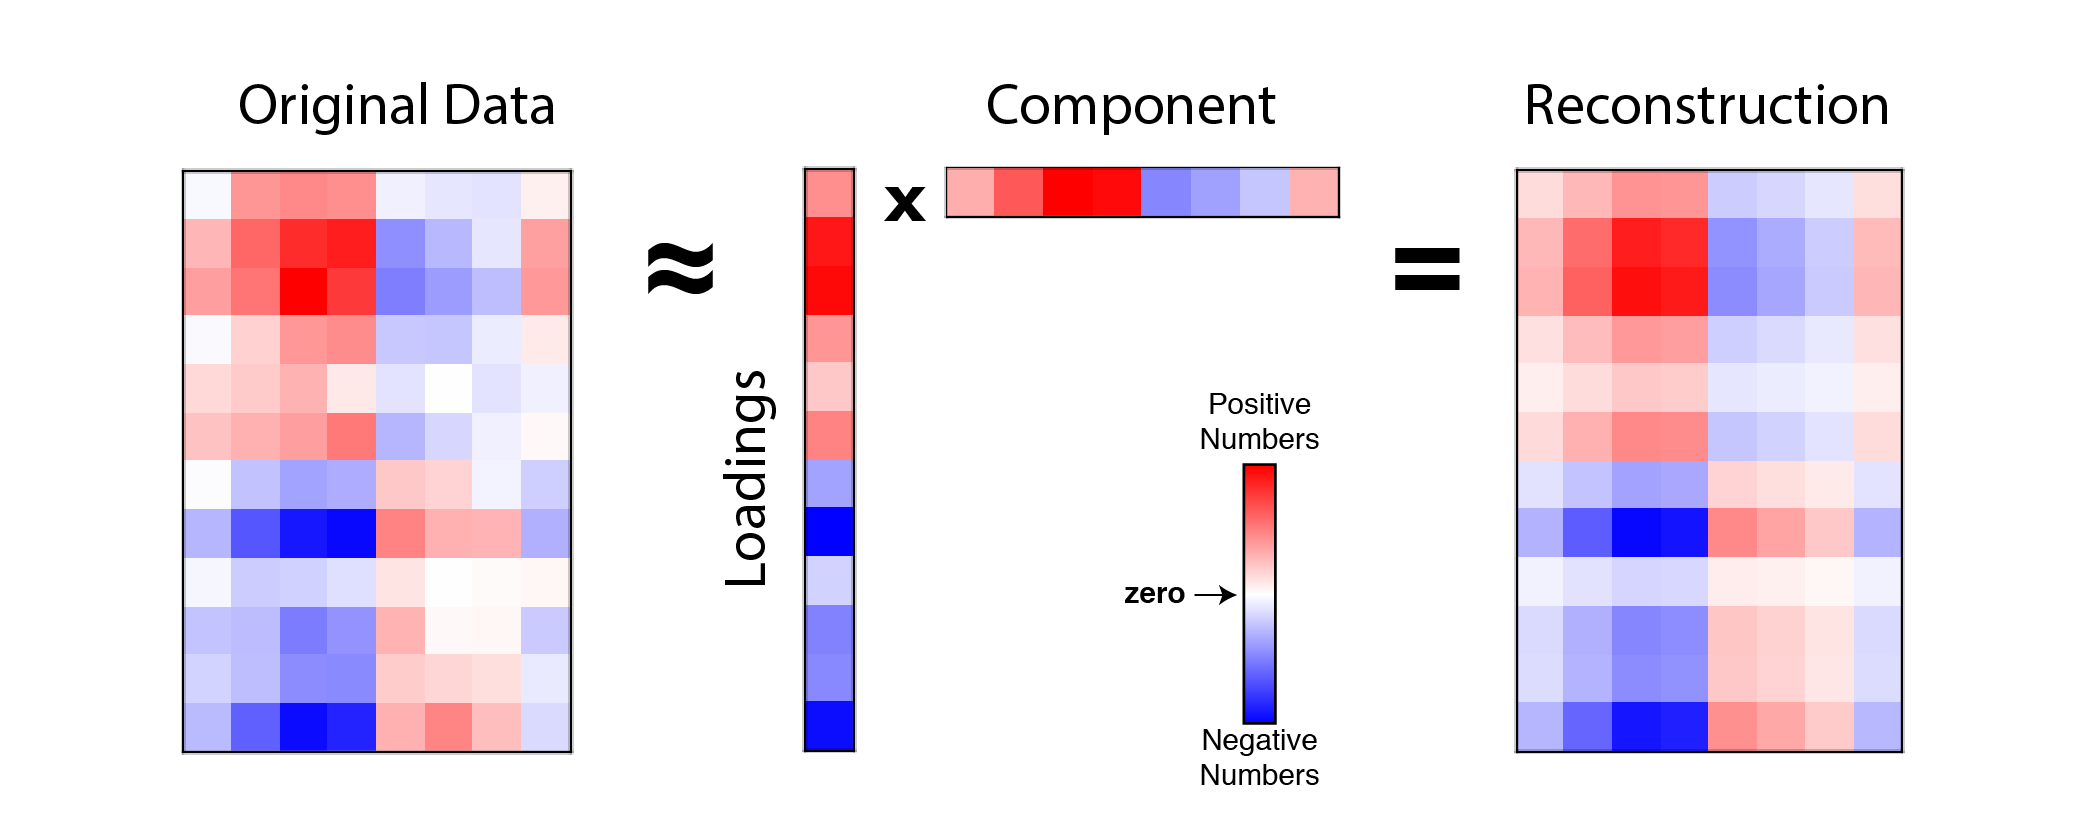
\includegraphics[width=10cm]{pics/recons-pcs.png}
    \end{figure}
\end{frame}

\begin{frame}{$L_1$主成分分析问题描述}
    \begin{itemize}
        \item
        $L_1$主成分分析问题描述
    \end{itemize}
    \small
    \begin{equation}\label{p3}
        P_3: \ 
    \hat{\bm{A}}_{p\times m}, \hat{\bm{F}}_{m\times n} = \underset{\bm{A},\bm{F}}{\operatorname{arg\ min} } \|\bm X - \bm{A}\bm{F}\|_{L_1}
    = \underset{\bm{A}, \bm{F}}{\operatorname{arg\ min}} \sum_{i=1}^p \sum_{j=1}^m |x_{ij} - \bm a_i^T \bm f_i|.
    \end{equation}
    \begin{equation}\label{p4}
        P_4: \ \hat{\bm A} = \underset{\bm{A}}{\operatorname{arg \ max}} \| \bm A^T \bm X\|_{L_1}
        = \underset{\bm A}{\operatorname{arg\ max}} 
        \sum_{i=1}^{n}\sum_{k=1}^{m}|\sum_{j=1}^p{a}_{jk}x_{ij}|
         \text{,其中}\bm A^T\bm A = \bm I_m
    \end{equation}
\end{frame}

\begin{frame}{一种$L_1$主成分分析的交替凸优化算法}
    \begin{itemize}
        \item
        Qifake \& Kande于2005年提出一种交替凸优化算法。
    \end{itemize} 
    \begin{table}[H]%%%%%%开始表格
        \tiny 
        \centering%把表居中
        \begin{tabular}{{p{0.9\columnwidth}}}%三个c代表该表一共三列,内容全部居中
        \toprule%第一道横线 表头
        交替凸优化求解$L_1$主成分分析 (ACP, Alternate Convex Programming) \\
        \midrule%第二道横线 符号+解释+单位 中间用&隔开
        1.初始化:给出$\bm{A}$,$\bm \Sigma$的初始值$\bm{A}^{(0)}$,$\bm \Sigma^{(0)} = \bm I$,(其中$\bm \Sigma$为一对角矩阵,
        $\bm I$为单位矩阵); \\
    
        2.交替凸优化:对于迭代次数$t = 1, ..., \tau$: \\
        $$ \bm F^{(t)} = \underset{\bm F}{\operatorname{arg\ min}} \|\bm X - \bm{A}^{(t-1)}\bm\Sigma^{(t-1)}\bm F^{T}\|_{L_1}$$ \\
        $$ \bm{A}^{(t)} = \underset{\bm{A}}{\operatorname{arg\ min}} \|\bm X - \bm{A}\bm\Sigma^{(t-1)}{(\bm F^{(t)})}^T \|_{L_1}$$ \\
        \begin{equation*}
            \text{归一化:}\left\{
                        \begin{array}{clr}
                        \bm N_a = diag({(\bm A^{(t)})}^T\bm{A}^{(t)})\\
                        \bm N_f = diag({(\bm F^{(t)})}^T\bm F^{(t)})\\
                        \bm F^{(t)} \leftarrow \bm F^{(t)}\bm N_f^{-1}\\
                        \bm{A}^{(t)}\leftarrow \bm{A}^{(t)}\bm N_a^{-1}\\
                        \bm \Sigma^{(t)} \leftarrow \bm N_a\bm \Sigma^{(t-1)}\bm N_f\\
                        \end{array}
            \right.
        \end{equation*} \\
    
        3.输出结果:$\bm{A} \leftarrow \bm{A}^{(\tau)}\bm \Sigma^{1/2}$,对$\bm{A}$进行QR分解取正交矩阵得到$\hat{\bm{A}}$;
        $\hat{\bm{F}} \leftarrow \hat{\bm{A}}^T\bm{X}$。 \\
        \bottomrule%第三道横线
        \end{tabular}
    \end{table}%%%%%%结束表格
\end{frame}

\begin{frame}{模拟实验准备}
    \begin{figure}[H]
        \centering
        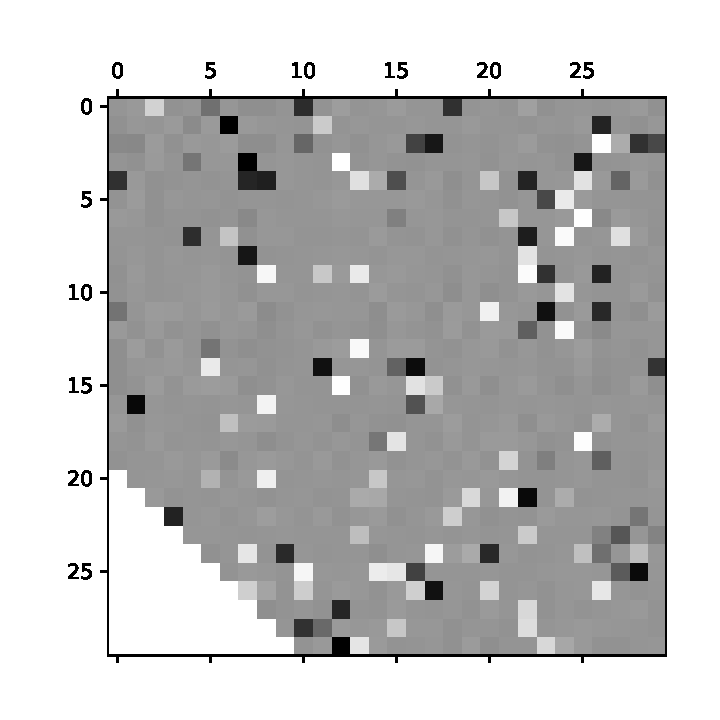
\includegraphics[width=.5\textwidth]{pics/matrix.pdf}
        \caption{\small $30\times30$的模拟矩阵}
        \label{fig2.1}
    \end{figure}
\end{frame}

\begin{frame}{模拟实验结果}
    \begin{figure}[H]
        \centering
        \begin{minipage}[t]{0.48\textwidth}
        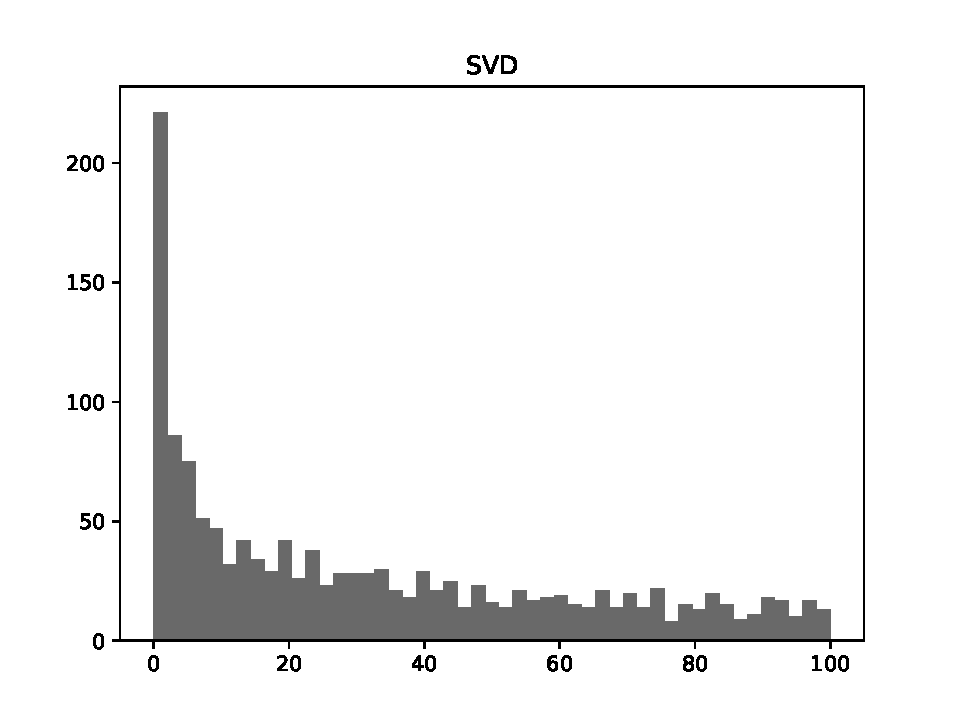
\includegraphics[width=5cm]{pics/svd.pdf}
        \end{minipage}
        \begin{minipage}[t]{0.48\textwidth}
        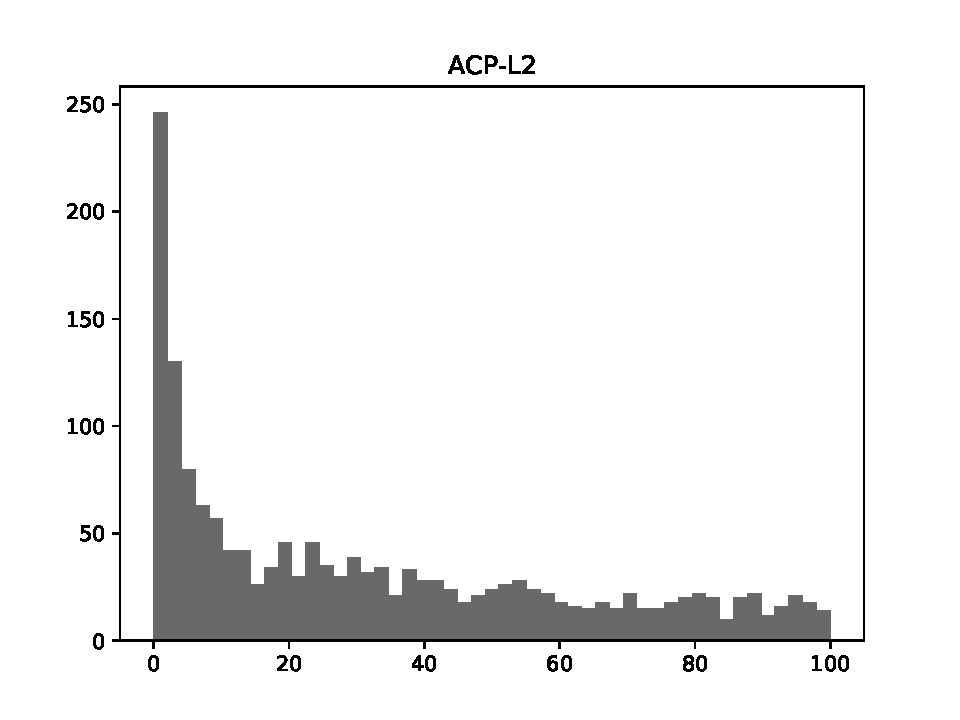
\includegraphics[width=5cm]{pics/acp-l2.pdf}
        \end{minipage}
        \begin{minipage}[t]{0.48\textwidth}
        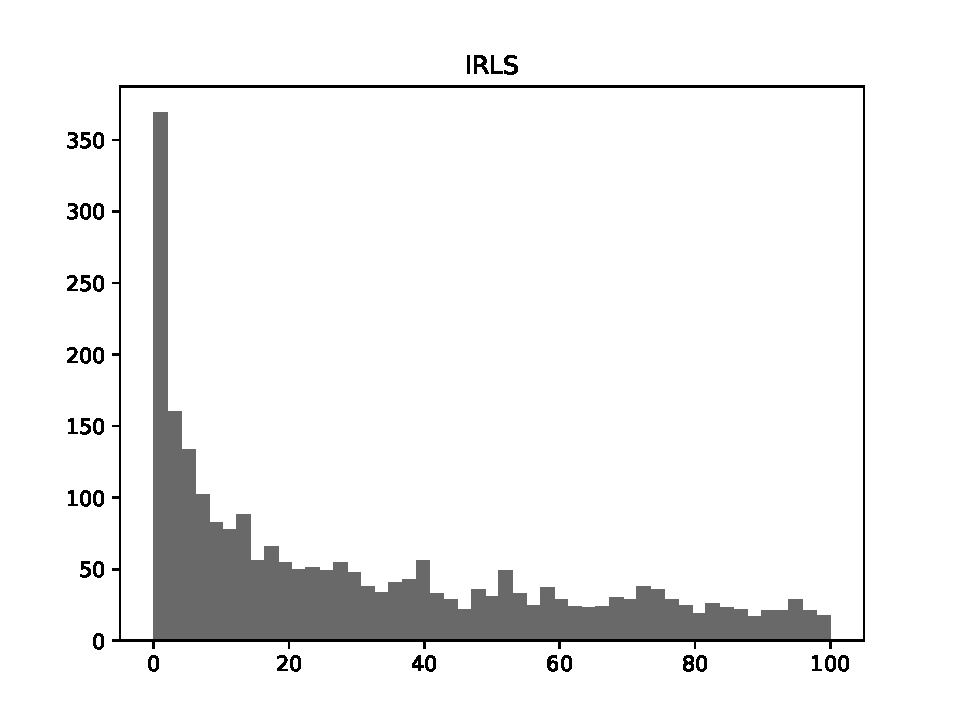
\includegraphics[width=5cm]{pics/IRLS.pdf}
        \end{minipage}
        \begin{minipage}[t]{0.48\textwidth}
        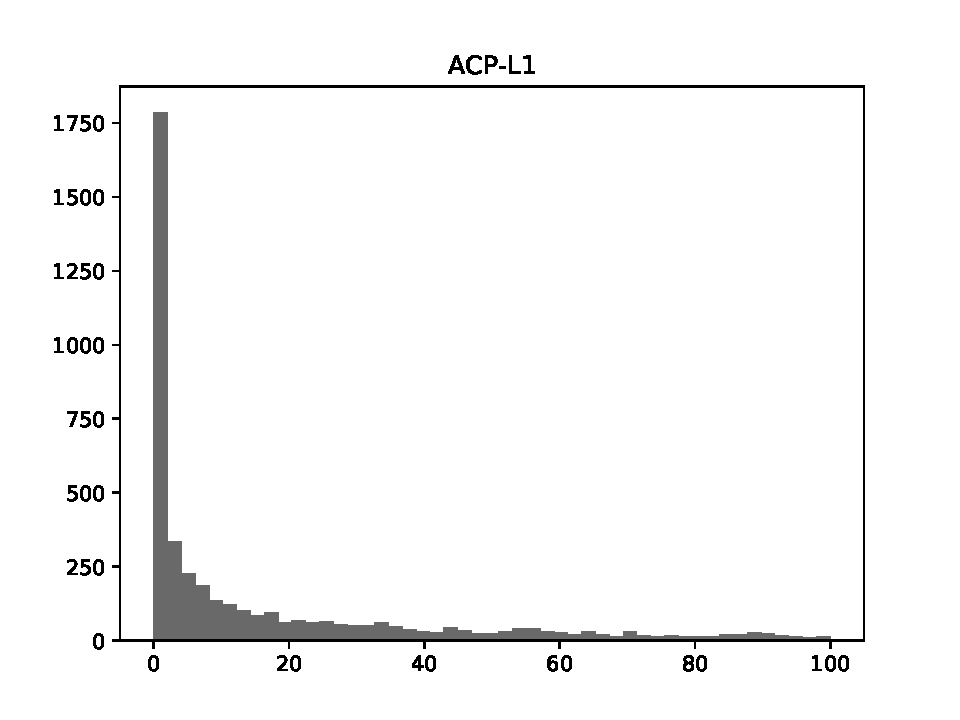
\includegraphics[width=5cm]{pics/acp-l1.pdf}
        \end{minipage}
    \end{figure}
\end{frame}

\begin{frame}{基于国内主要月度宏观经济数据的实证研究}
    \begin{itemize}
        \item
        数据来源:EPS数据平台-全国月度宏观经济数据
    \end{itemize}
    \begin{figure}[H]
        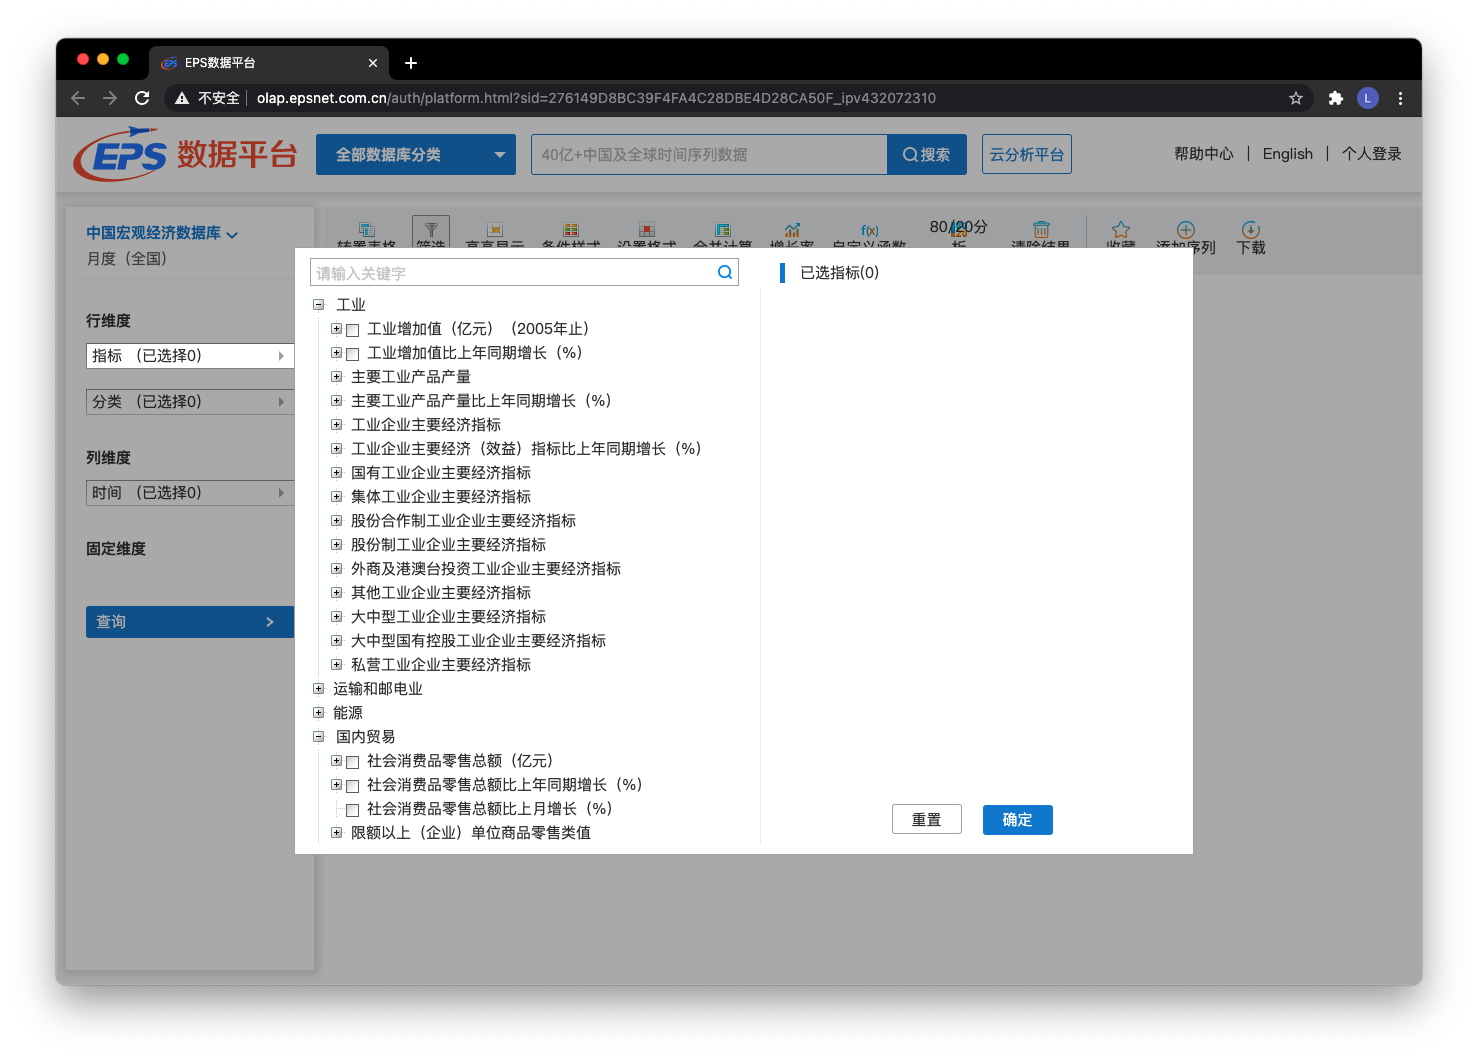
\includegraphics[width=9cm]{pics/data-source.png}
    \end{figure}
\end{frame}

\begin{frame}{基于国内主要月度宏观经济数据的实证研究}
    \begin{itemize}
        \item
        宏观经济数据的重尾性
    \end{itemize}
    \begin{figure}[H]
        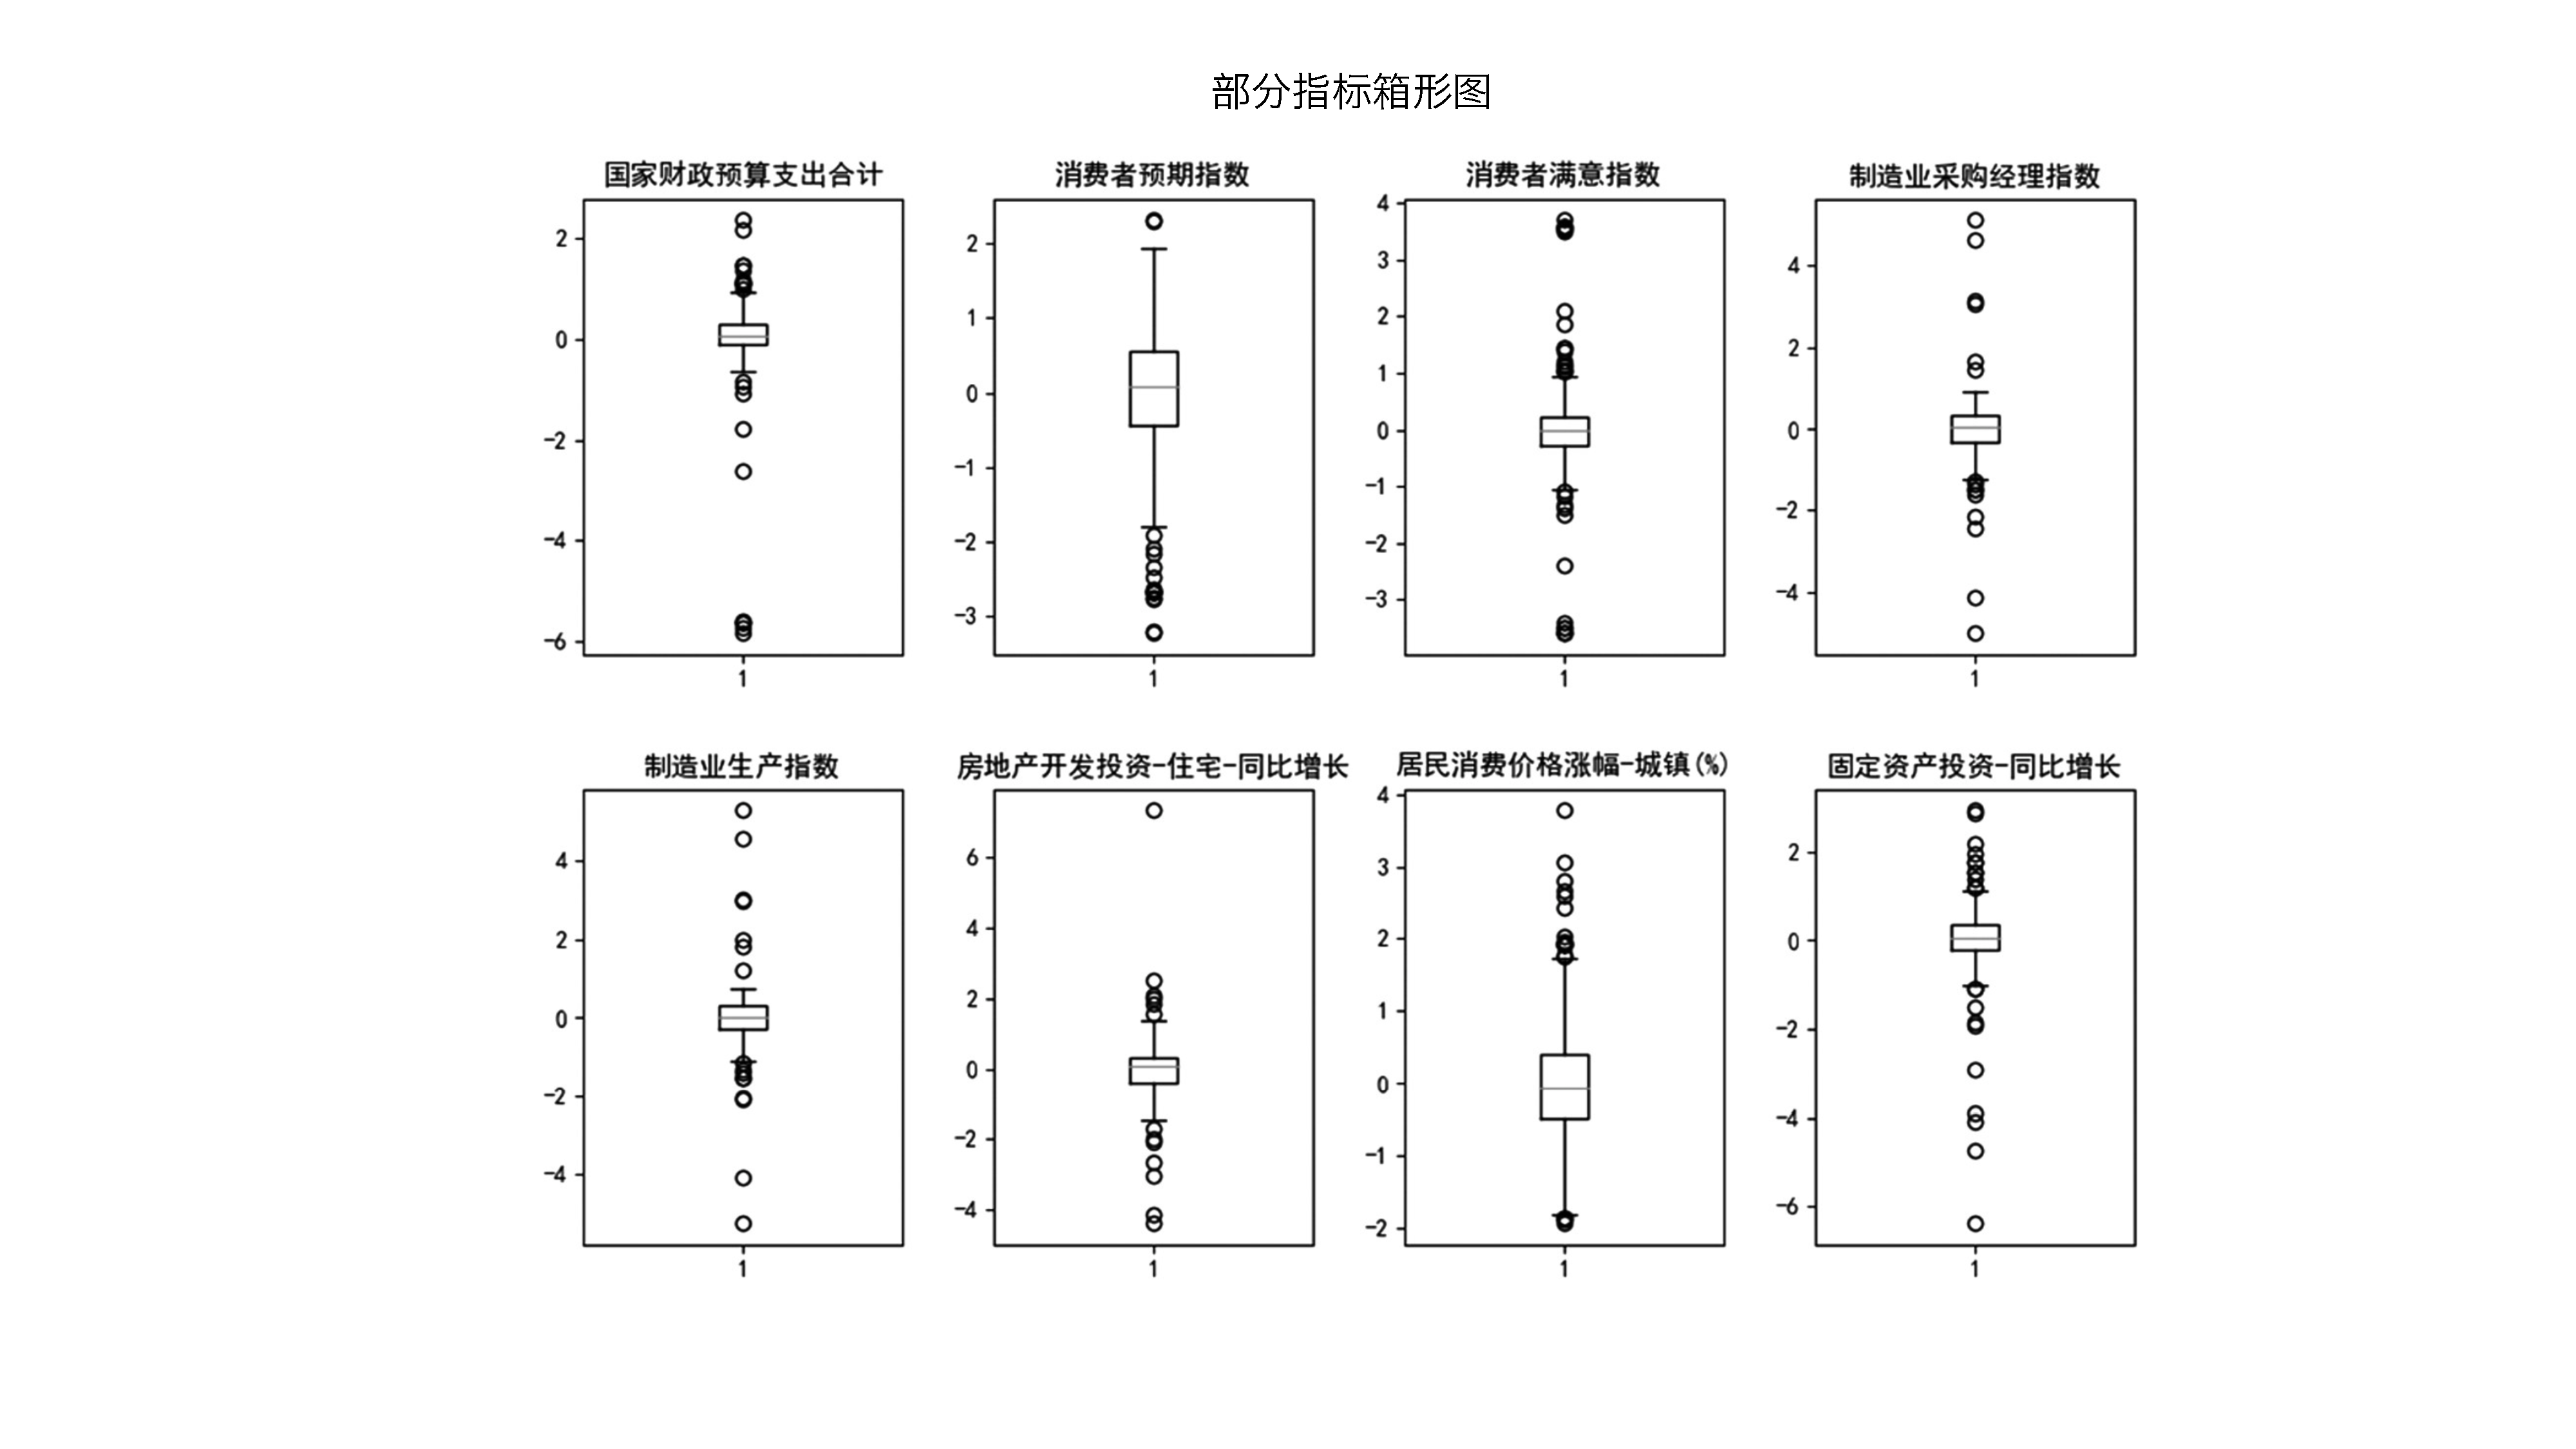
\includegraphics[width=10cm]{pics/box.pdf}
    \end{figure}
\end{frame}

\begin{frame}{基于国内主要月度宏观经济数据的实证研究}
    \begin{itemize}
        \item
        宏观经济数据的重尾性
    \end{itemize}
    \begin{figure}[H]
        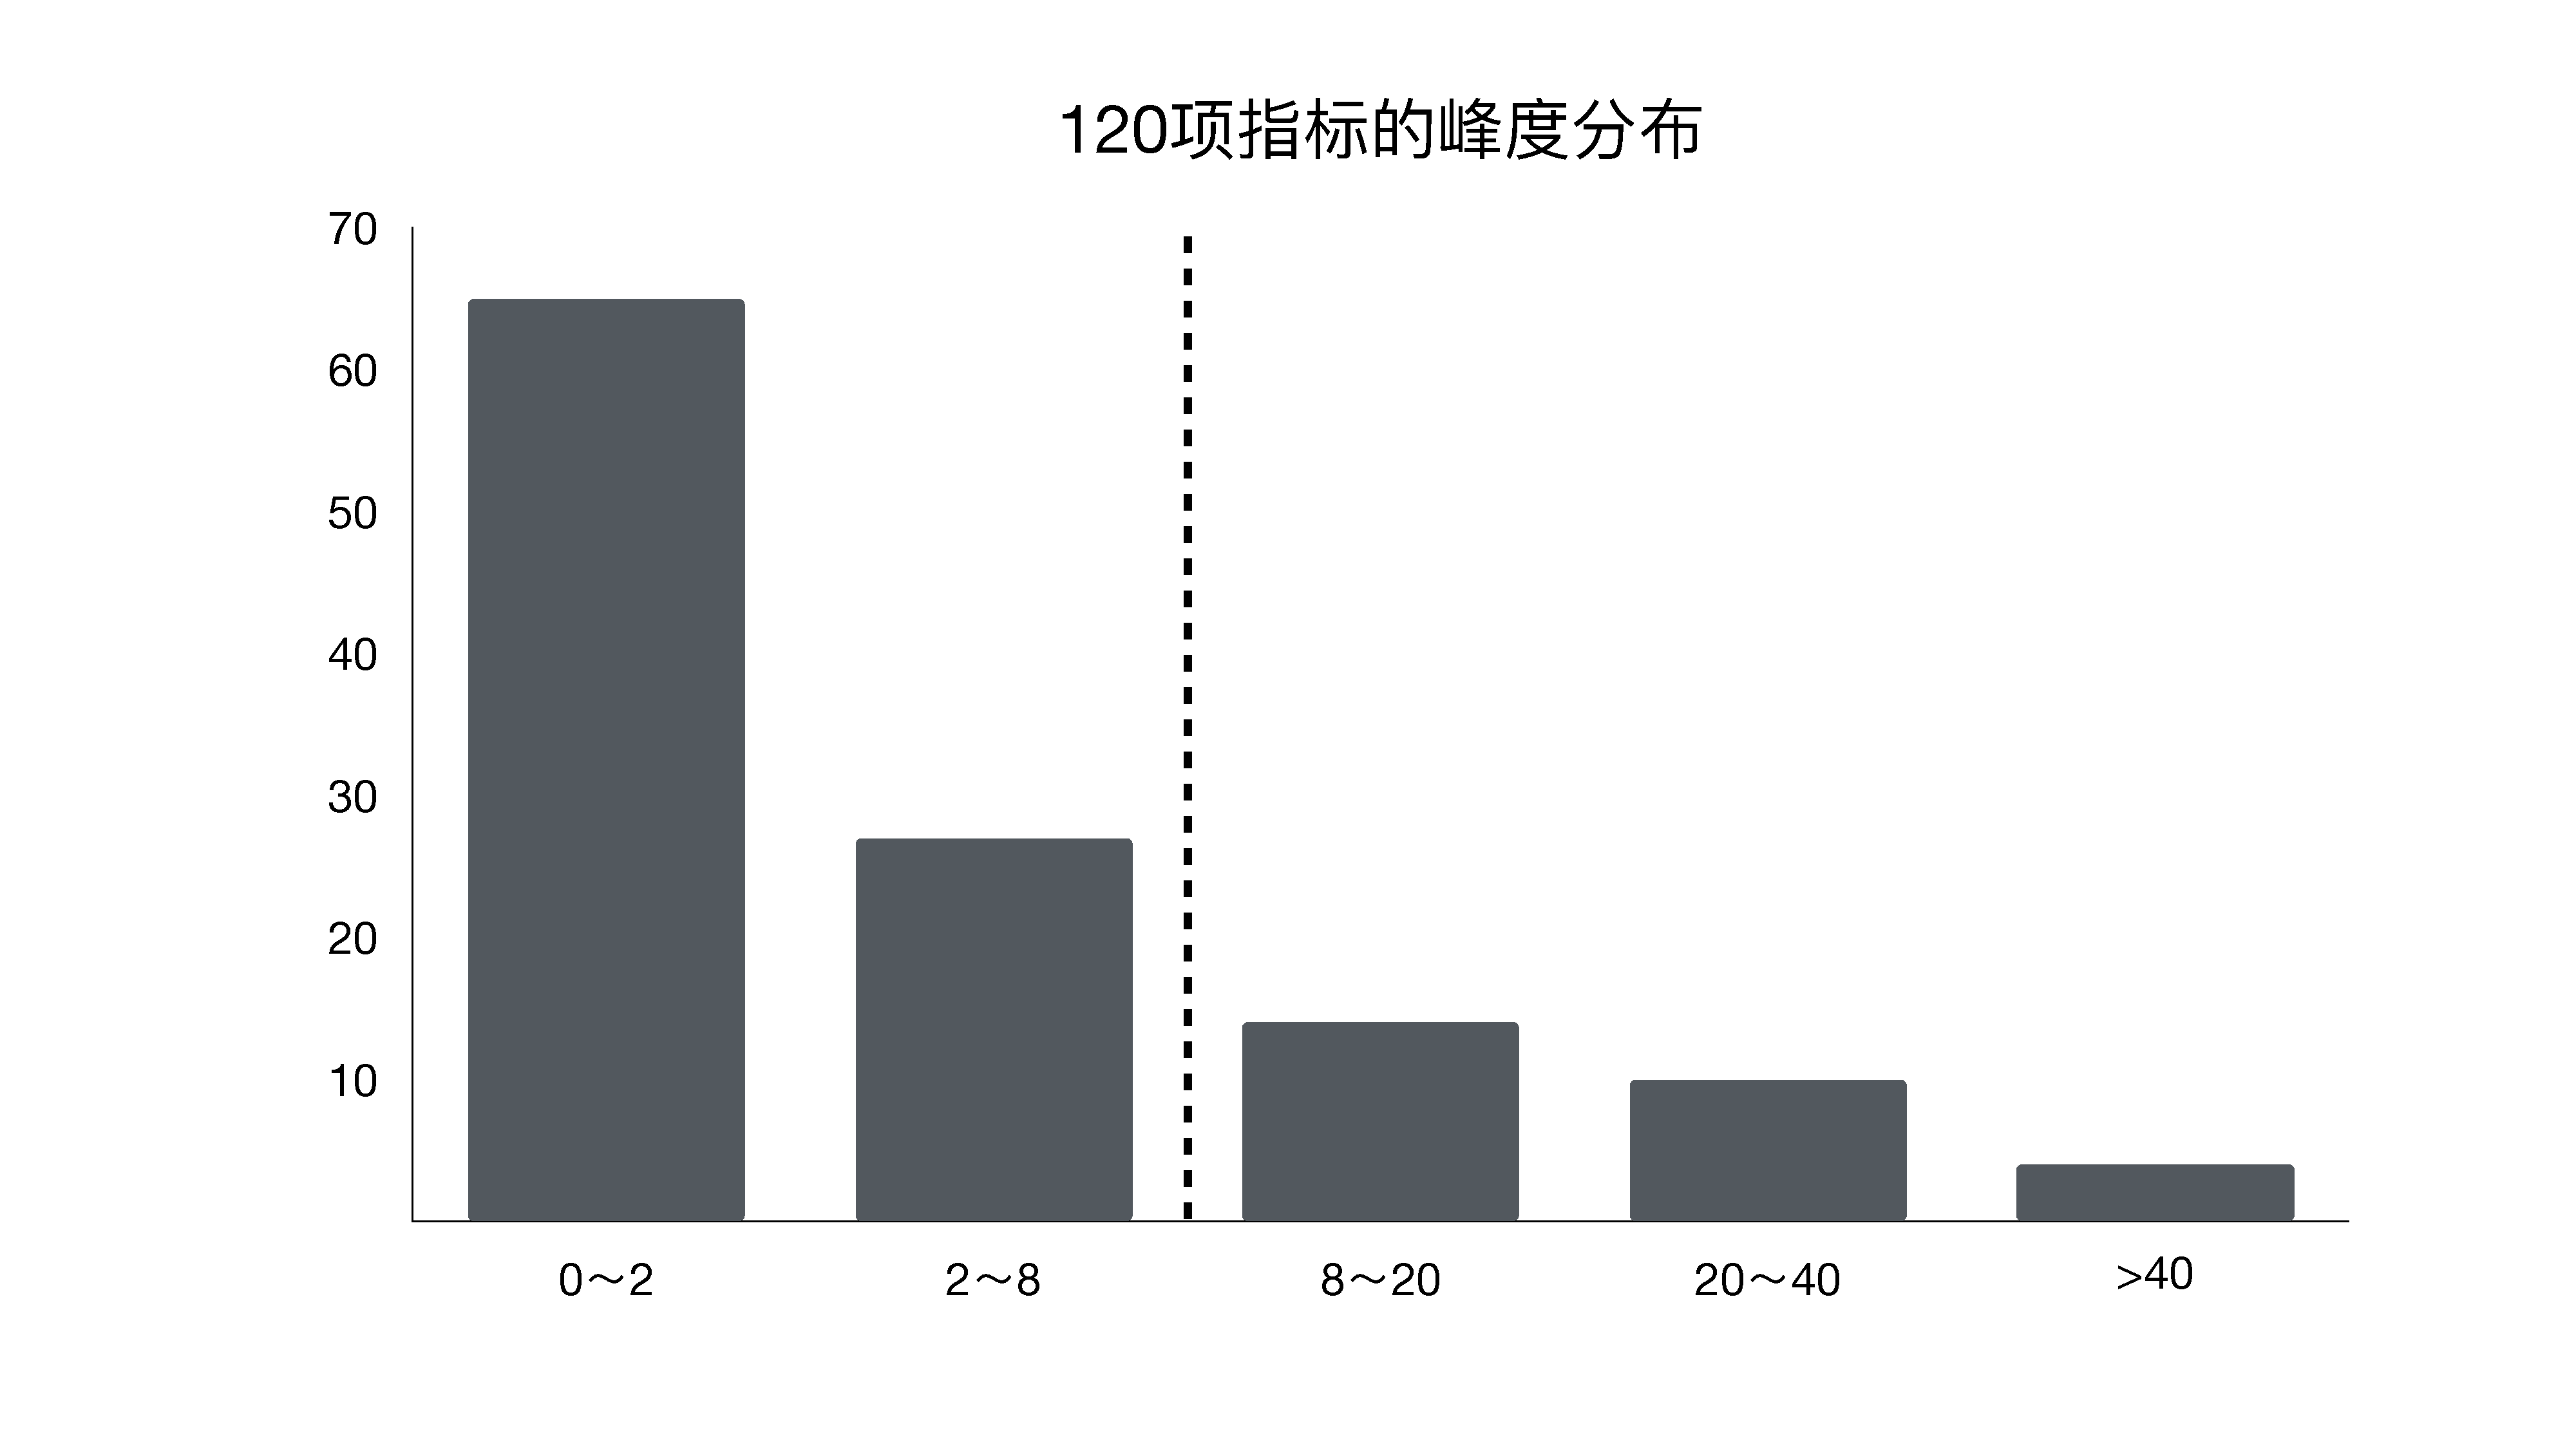
\includegraphics[width=10cm]{pics/skew.pdf}
    \end{figure}
\end{frame}

\begin{frame}{利用扩散指数模型进行预测}
    \begin{itemize}
        \item
        扩散指数模型预测
    \end{itemize}
\begin{equation}
    \bm{X}_t = \bm{A}\bm{F}_t + \bm{e}_t
\end{equation}
\begin{equation}\label{predict-factor-model}
    y_{t+h} = \bm{\beta}(L)\bm{F}_t + \bm{\alpha}(L)y_t + c + e_{t+h}
\end{equation}
\begin{itemize}
    \item
    因子个数选择,Bai\&Ng信息准则。
\end{itemize}
\end{frame}

\begin{frame}{利用扩散指数模型进行预测}
    \begin{itemize}
        \item
        滑动窗口预测
    \end{itemize}
    \begin{figure}[H]
        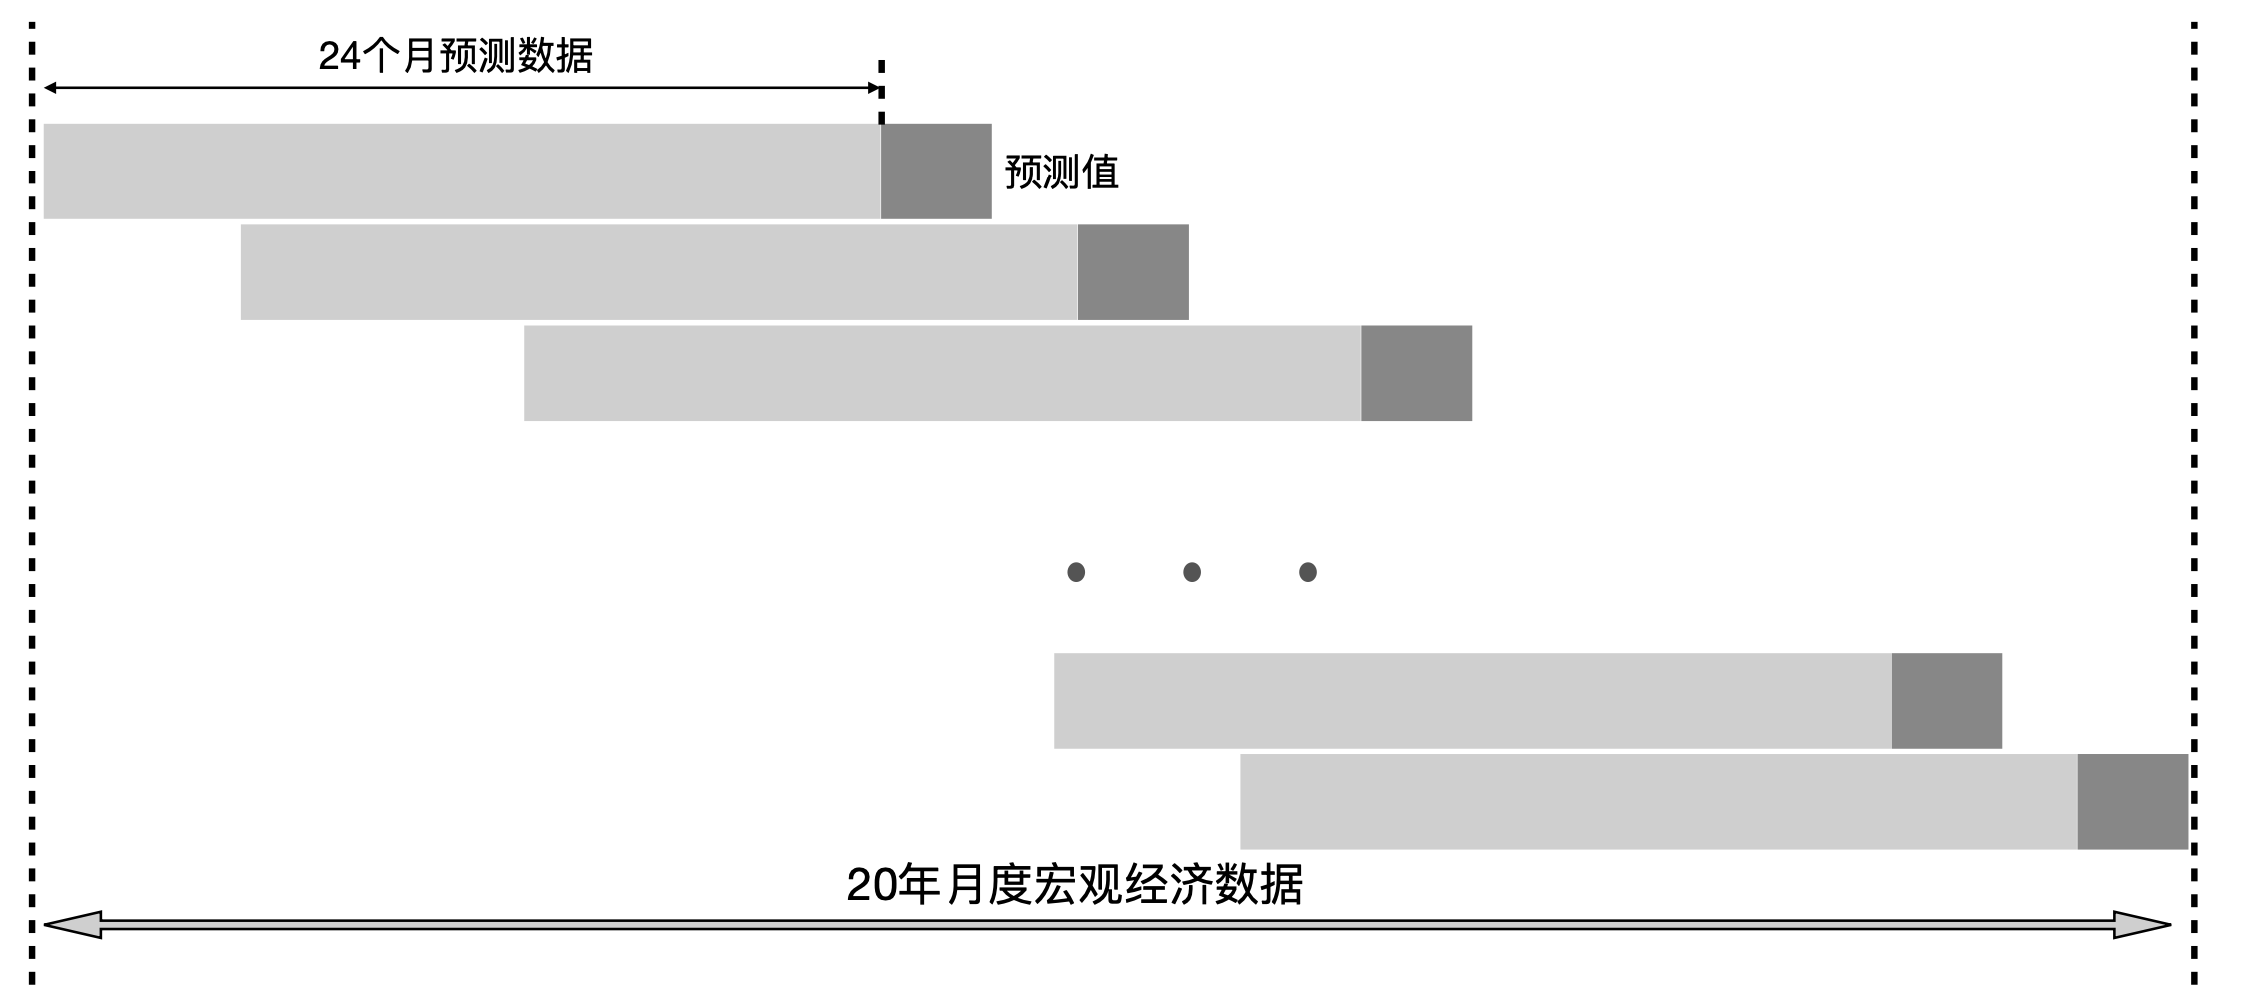
\includegraphics[width=10cm]{pics/predict.png}
    \end{figure}
\end{frame}

\begin{frame}{实证结果}
    \begin{itemize}
        \item
        预测结果表明:$L_1$因子在短期预测中比$L_2$因子更准确。
        长期预测,表现也良好。
    \end{itemize}
    \begin{table}[H]
        \tiny
        \caption{向前一个月预测结果}
        \label{outcome1}
        \centering
        \begin{tabularx}{\textwidth}{lXXXXXX}
        \toprule
                         &  MSE(L1 PCA) &  MSE(IM) &  MAE(L1 PCA) &  MAE(IM) &  MPAE(L1 PCA) &  MPAE(IM) \\ \midrule
        消费者满意指数*     & 0.81            & 1.49        & 0.87            & 1.67        & 0.43             & 1.55         \\
        工业生产者出厂价格指数* & 0.70            & 1.98        & 0.75            & 1.54        & 0.96             & 1.60         \\
        货币供应量M2*      & 0.76            & 1.25        & 0.90            & 1.19        & 0.45             & 0.97         \\
        固定资产投资总额*  & 0.89            & 1.03        & 0.97            & 0.99        & 0.81             & 1.32         \\
        房地产开发投资总额* & 0.79            & 0.98        & 0.95            & 1.00        & 0.91             & 1.20         \\
        社会消费品零售总额* & 0.84            & 1.25        & 0.87            & 1.12        & 0.45             & 1.17         \\
        制造业采购经理指数    & 1.24           & 1.69        & 1.06            & 1.43        & 0.90             & 1.50         \\
        住宅新开工面积总数*  & 0.89            & 2.40        & 0.85            & 1.98        & 0.45             & 2.22         \\
        股票流通市值*      & 0.99            & 3.99        & 0.98            & 2.84        & 0.81             & 4.51         \\
        消费者信心指数*     & 0.93            & 1.01        & 0.98            & 0.99        & 0.98             & 1.56         \\ \bottomrule
        \end{tabularx}
    \end{table}
\end{frame}

\section{最小绝对值回归性能优化}

\begin{frame}{交替凸优化算法的计算性能问题}
    \begin{itemize}
        \item
        交替凸优化算法需要求解多个最小绝对值回归问题,
        在变量较多情况下,线性规划算法计算性能较差。
    \end{itemize}
\begin{figure}[H]
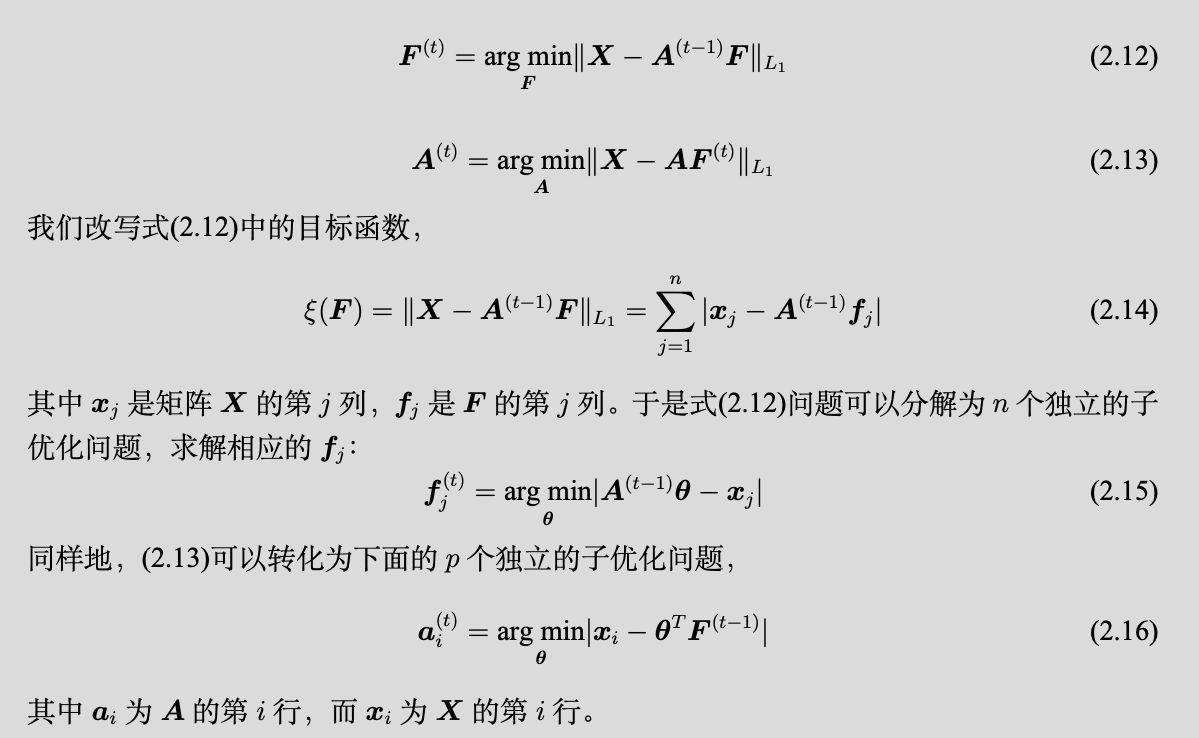
\includegraphics[width=8cm]{pics/acp-problem.png}
\end{figure}
\end{frame}

\begin{frame}{最小绝对值回归的优化1: 聚类——迭代拆解算法}
    \begin{itemize}
        \item
        Park等人于2016年提出一种聚类——迭代拆解算法,通过减小问题规模来提升计算性能。
    \end{itemize}
\begin{figure}[H]
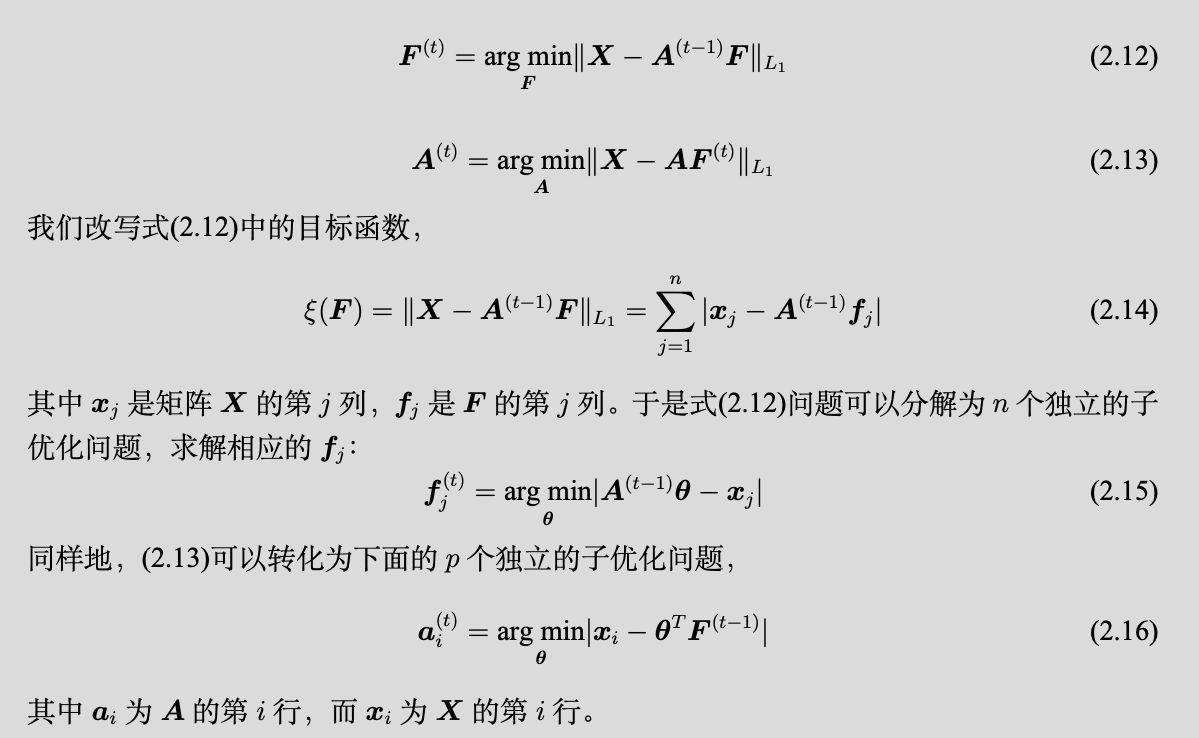
\includegraphics[width=8cm]{pics/acp-problem.png}
\end{figure}

\end{frame}
\begin{frame}{最小绝对值回归的优化1: 聚类——迭代拆解算法}
    \begin{itemize}
        \item 初始聚类,使用任意聚类方法,我们这里使用K-means。
    \end{itemize}
\begin{figure}[H]
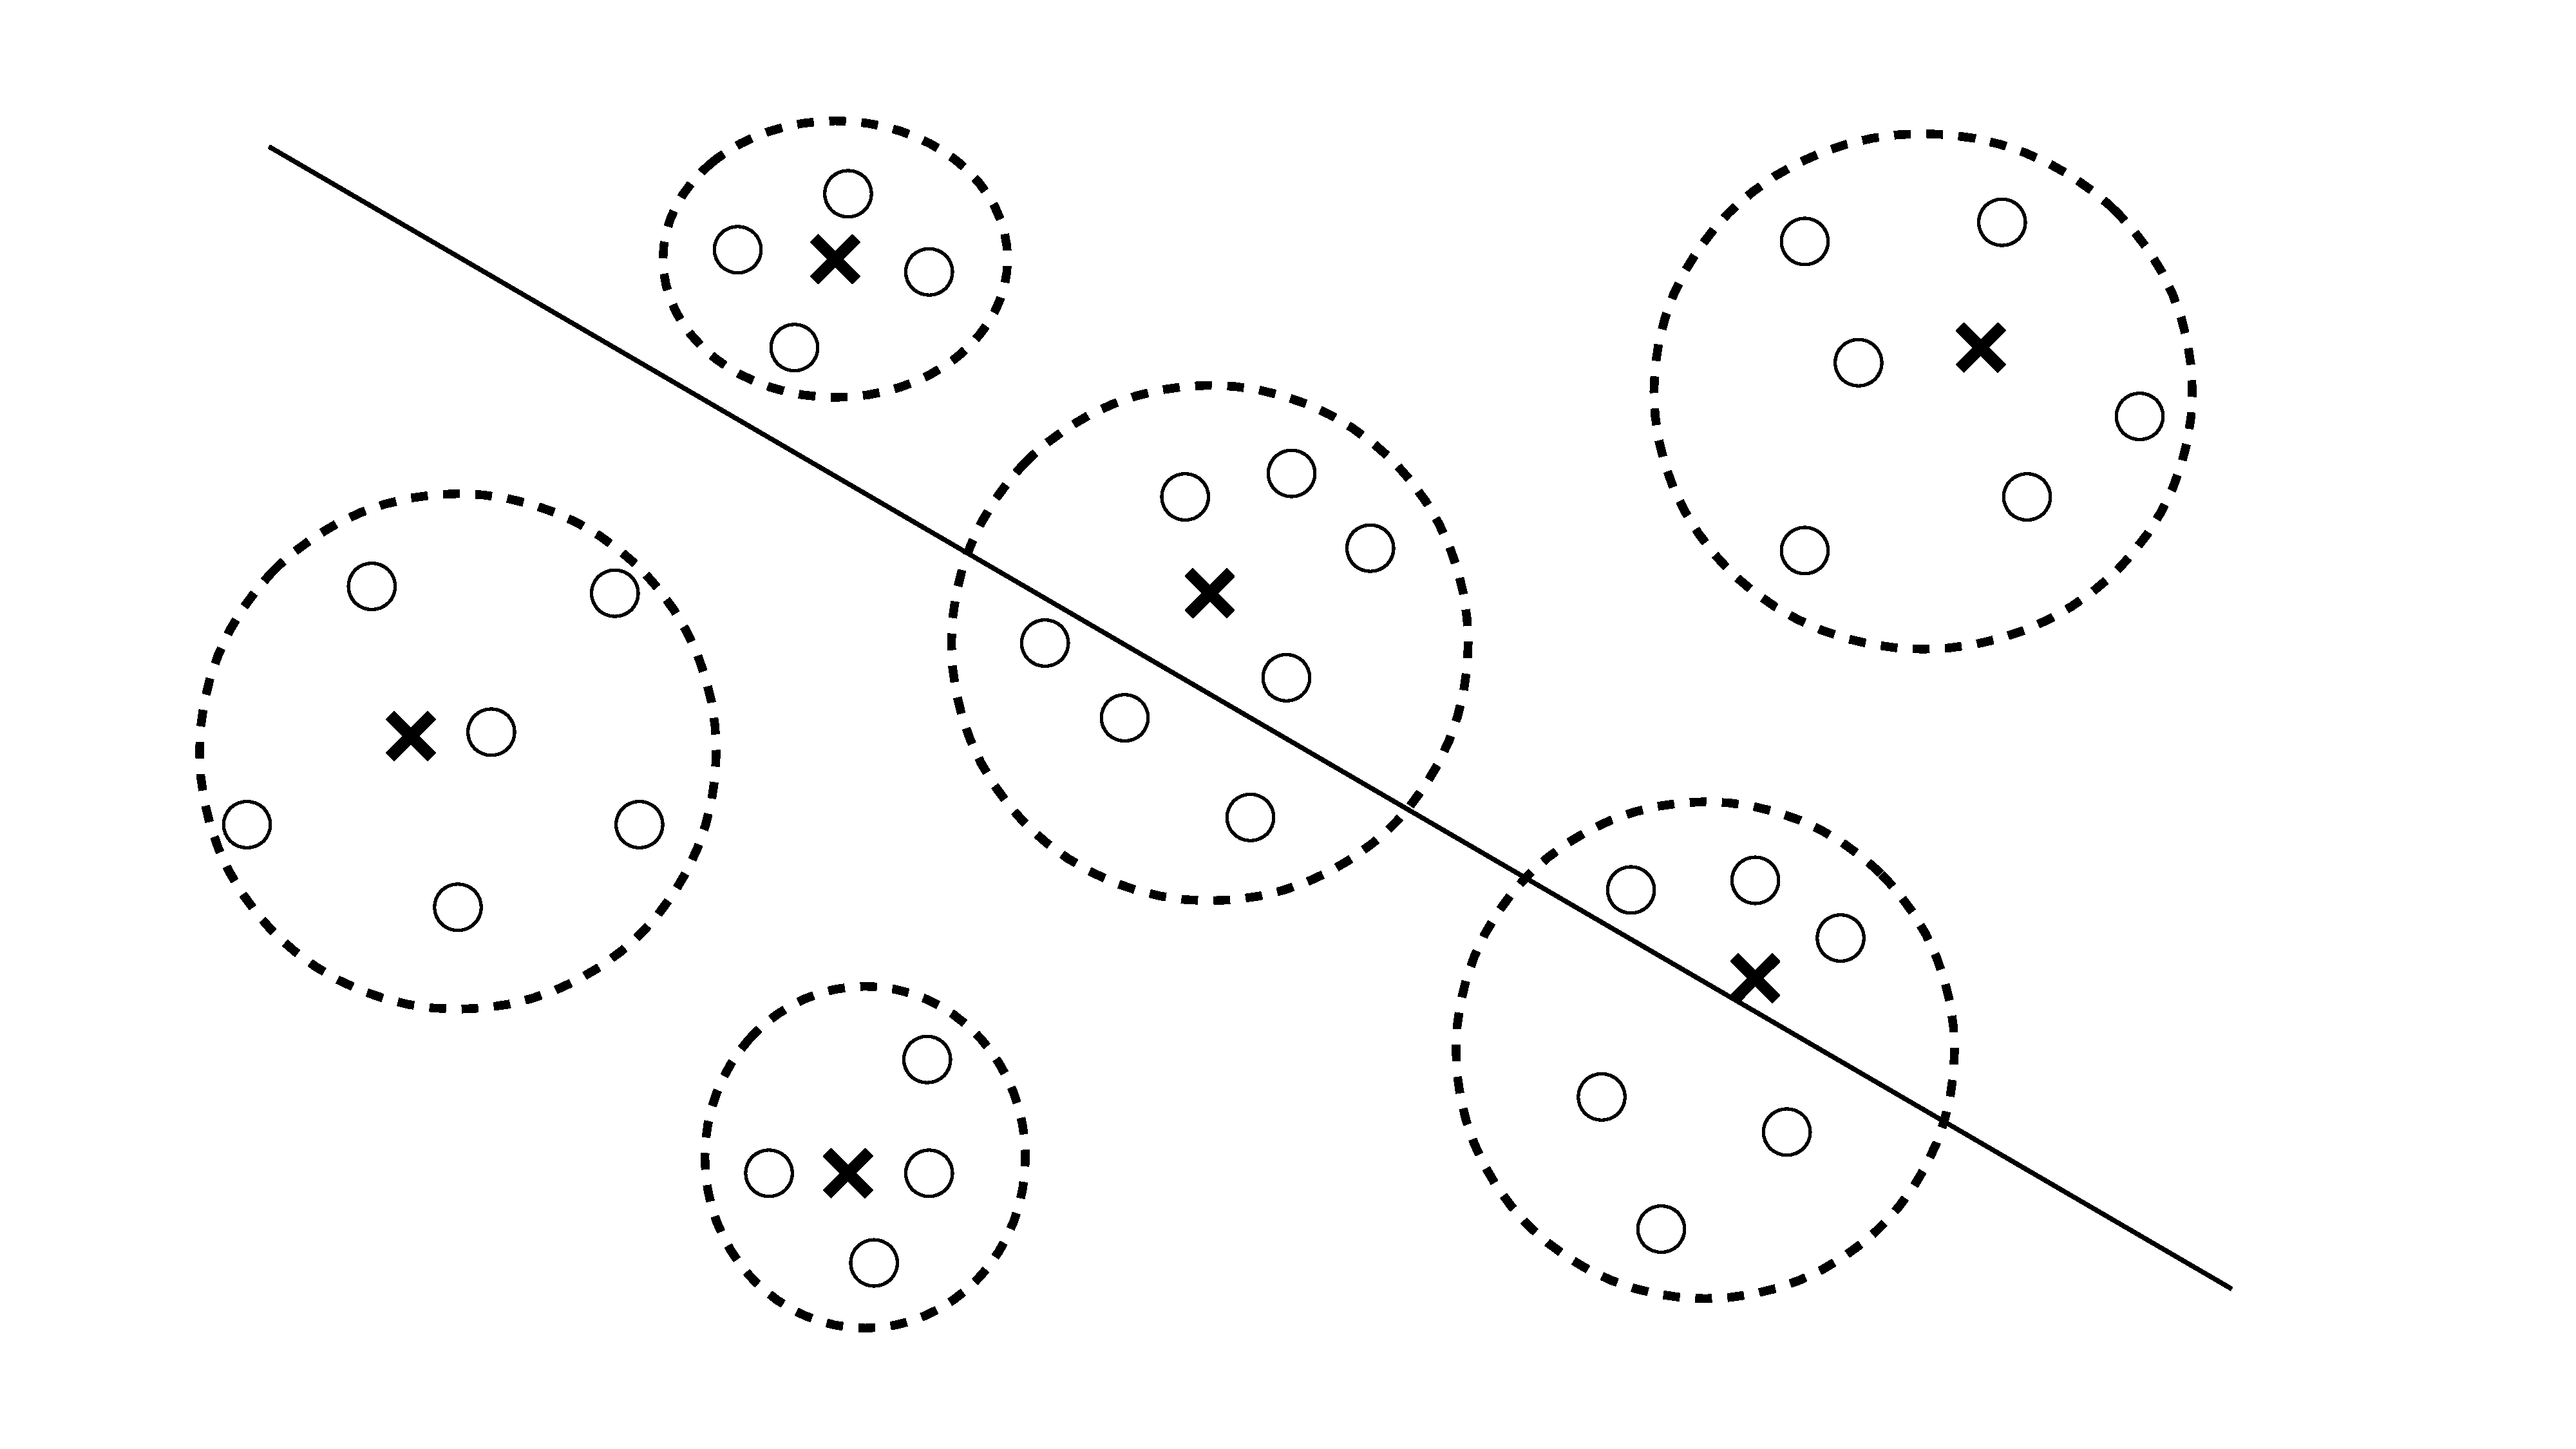
\includegraphics[width=10cm]{pics/aid-demo-a.pdf}
\end{figure}
\end{frame}

\begin{frame}{最小绝对值回归的优化1: 聚类——迭代拆解算法}
    \begin{itemize}
        \item 计算$\bm \beta$,按规则对聚类进行拆解。
    \end{itemize}
\begin{figure}[H]
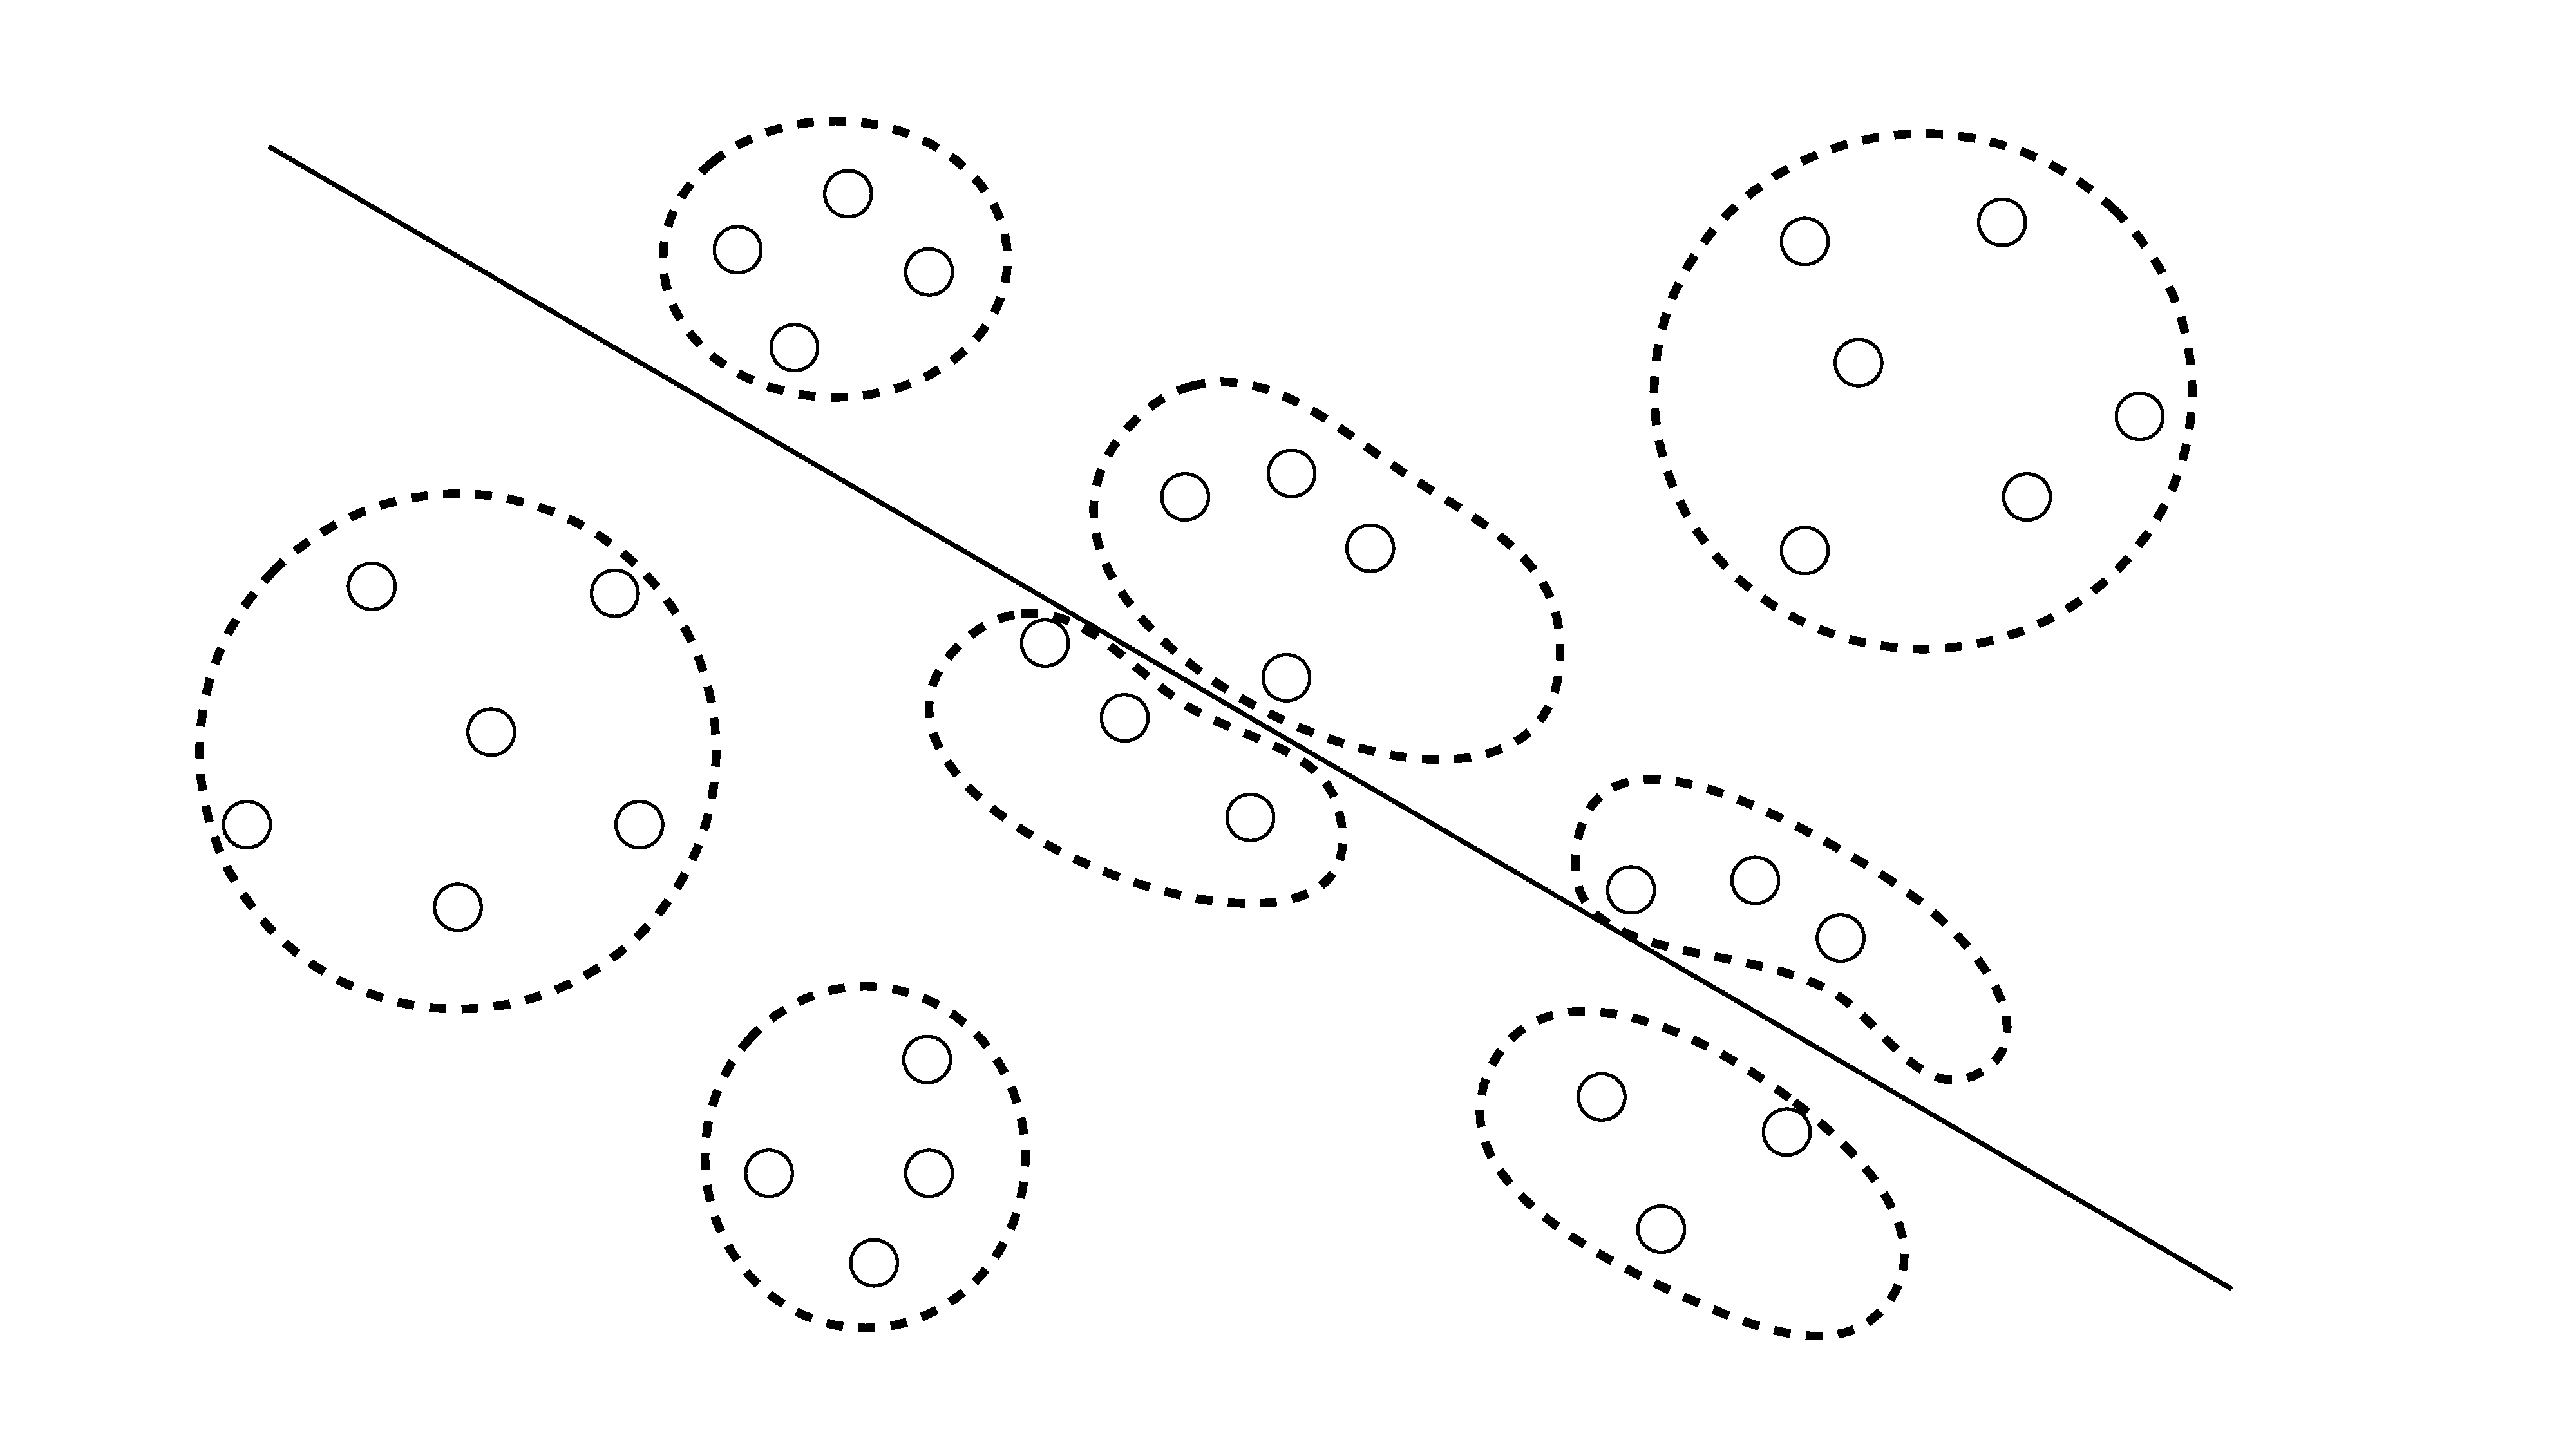
\includegraphics[width=10cm]{pics/aid-demo-b.pdf}
\end{figure}
\end{frame}

\begin{frame}{最小绝对值回归的优化1: 聚类——迭代拆解算法}
    \begin{itemize}
        \item 在新的聚类上重新计算$\bm \beta$。
    \end{itemize}
\begin{figure}[H]
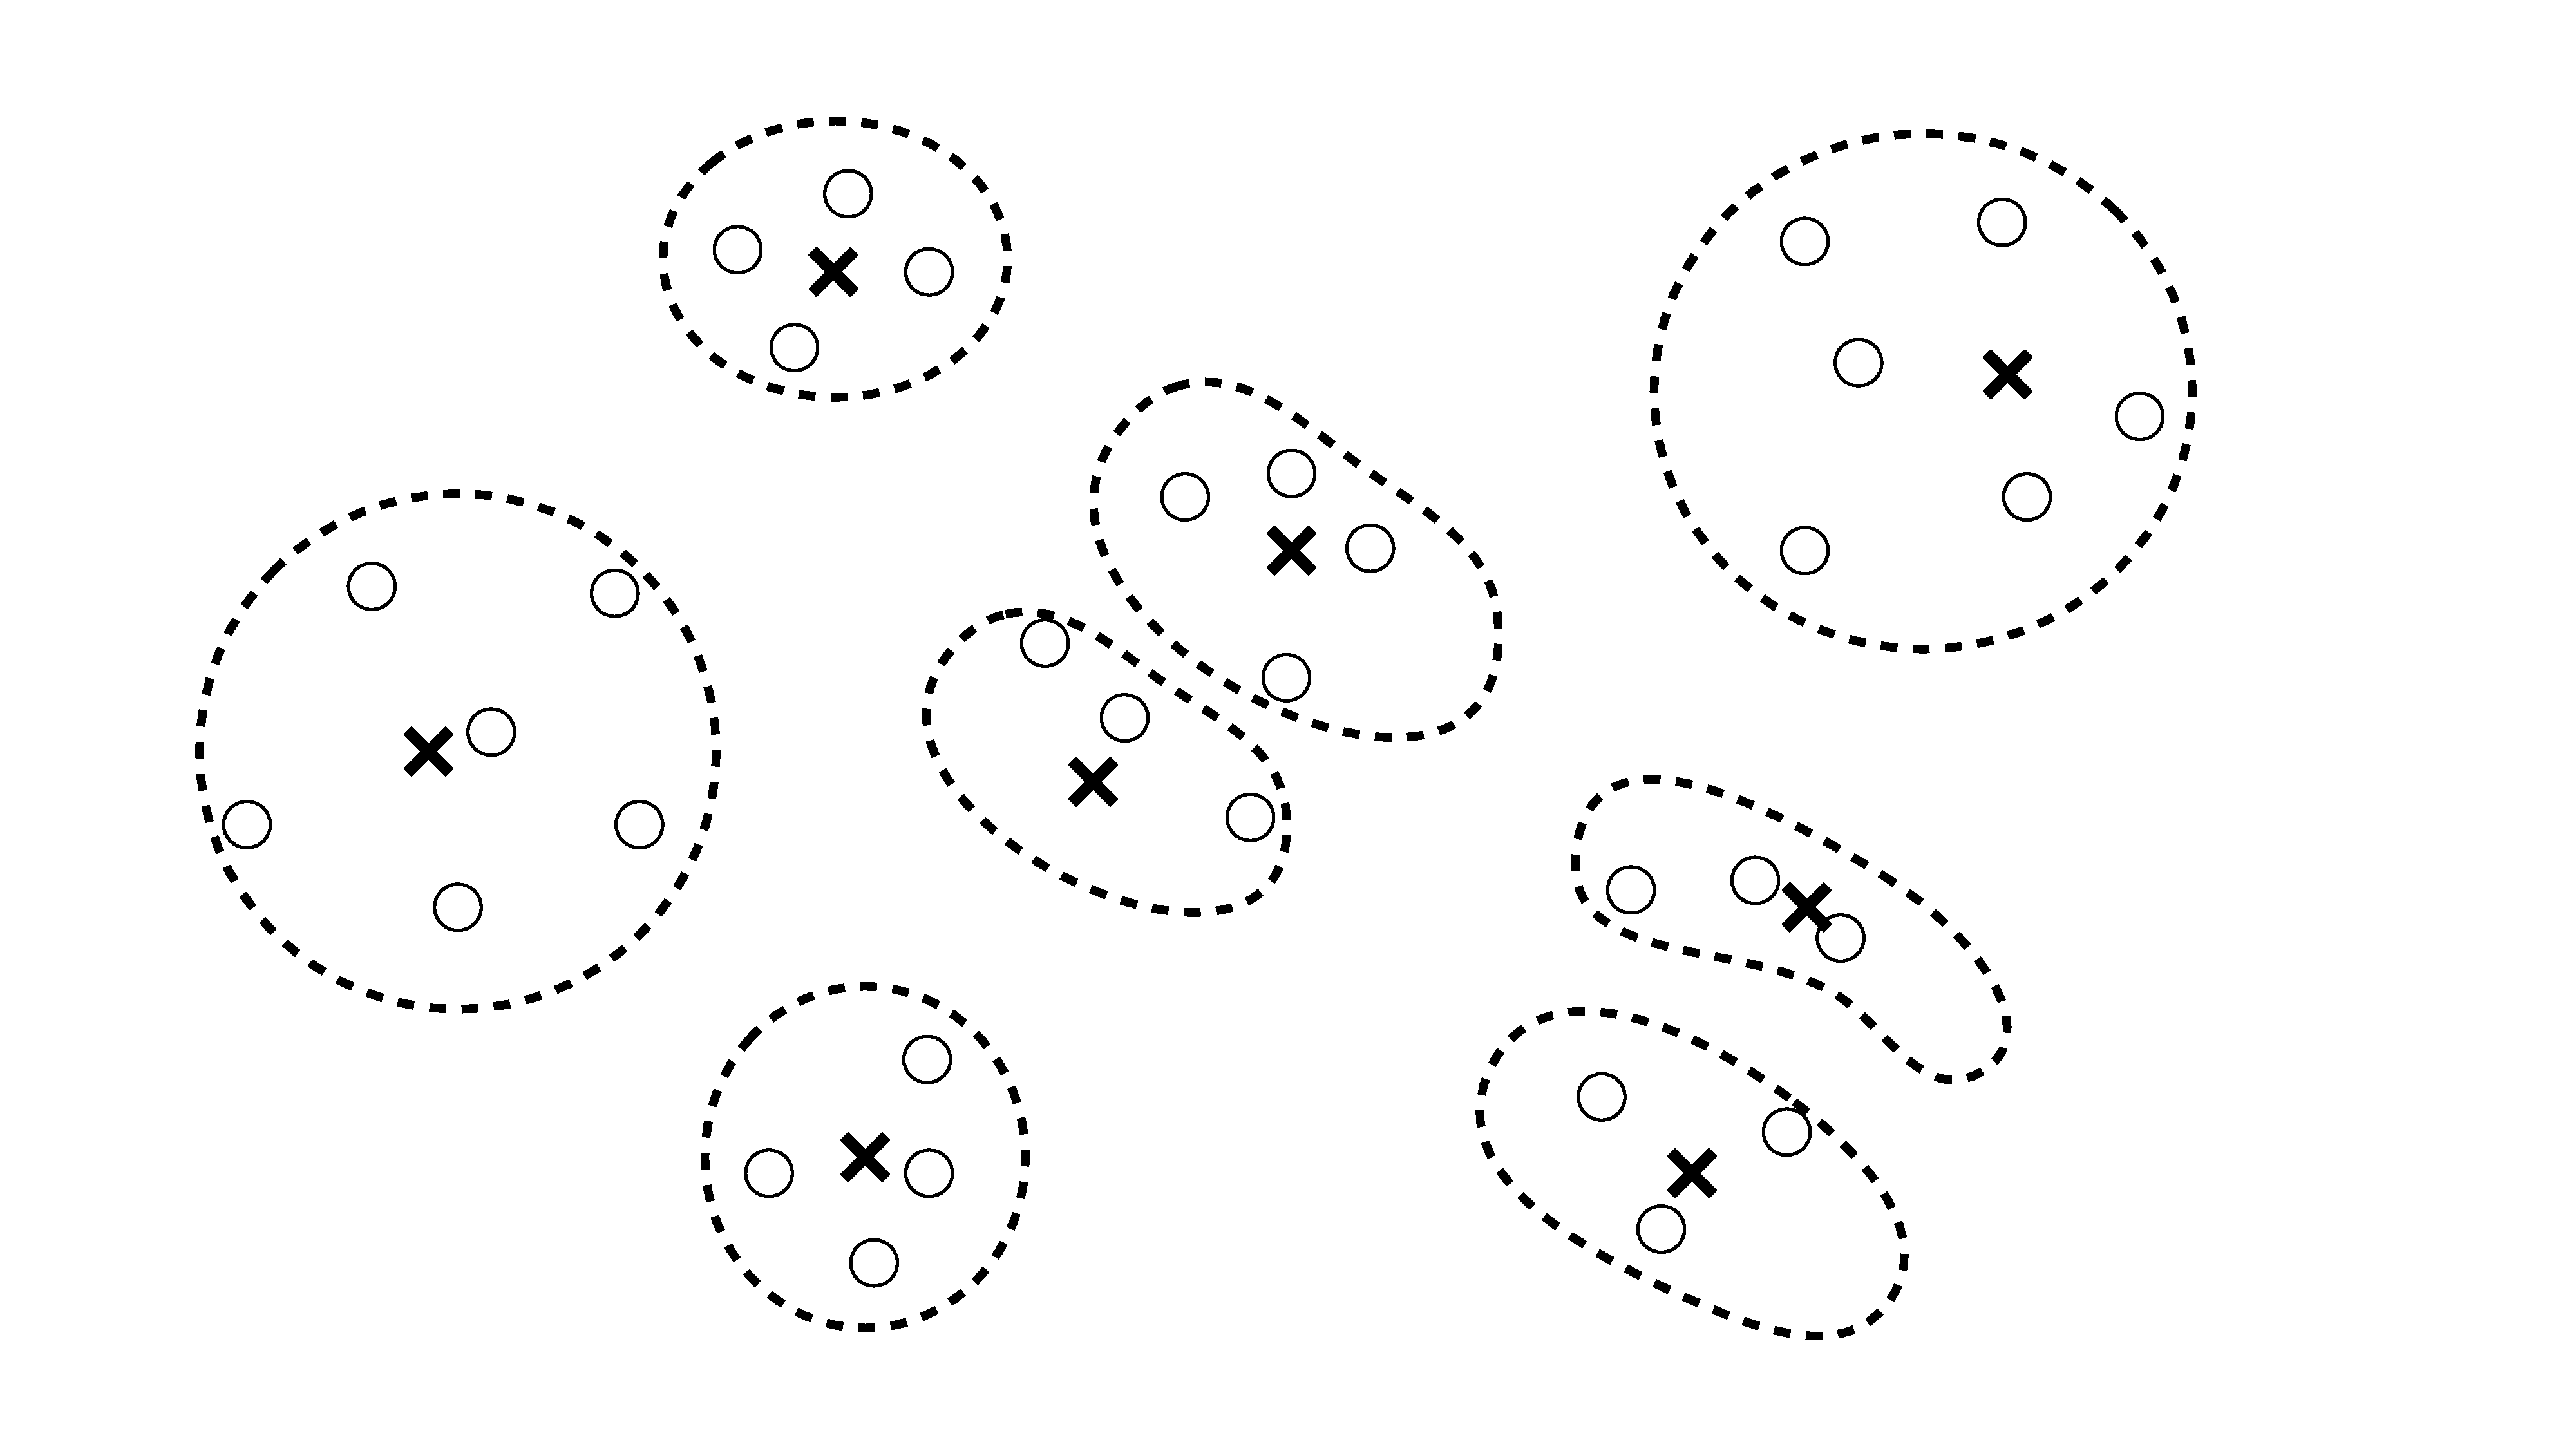
\includegraphics[width=10cm]{pics/aid-demo-c.pdf}
\end{figure}
\end{frame}

\begin{frame}{最小绝对值回归的优化1: 聚类——迭代拆解算法}
    \begin{itemize}
        \item 可以证明,该方法最终获得原问题的最优解
        (和在全部数据上解原优化问题有相同的解)。
    \end{itemize}
\begin{figure}[H]
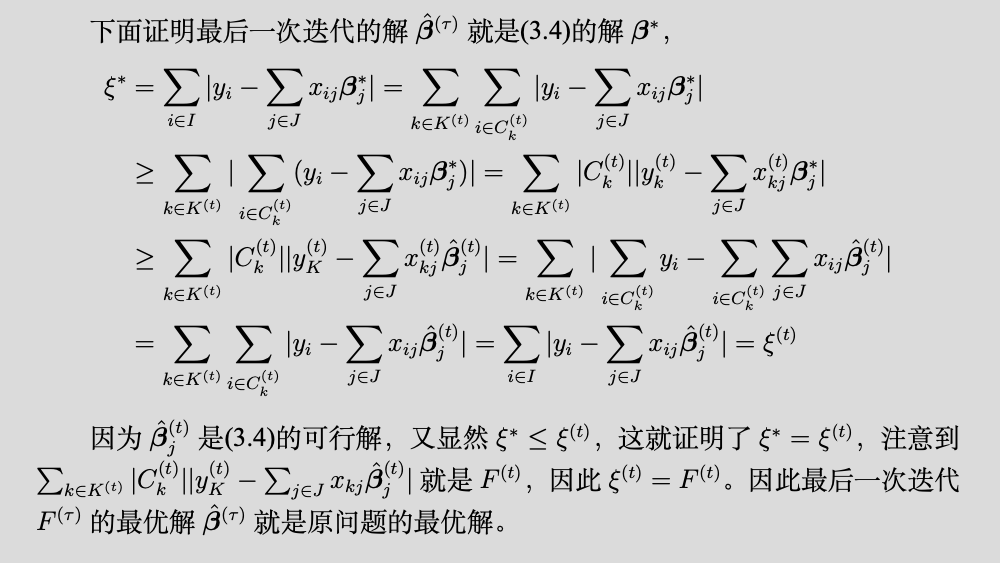
\includegraphics[width=10cm]{pics/proof-aid.png}
\end{figure}
\end{frame}

\section{另一种$L_1$主成分分析}

\begin{frame}{一种最大化特征空间投影$L_1$范数的贪婪算法}
    \begin{itemize}
        \item 交替凸优化算法可以解决问题$P_3$,问题$P_4$也是$L_1$主成分分析。
        \item 回顾$P_4$问题的表述:
    \end{itemize} 
    \small
    \begin{equation}\label{p4}
        P_4: \ \hat{\bm A} = \underset{\bm{A}}{\operatorname{arg \ max}} \| \bm A^T \bm X\|_{L_1}
        = \underset{\bm A}{\operatorname{arg\ max}} 
        \sum_{i=1}^{n}\sum_{k=1}^{m}|\sum_{j=1}^p{a}_{jk}x_{ij}|
         \text{,其中}\bm A^T\bm A = \bm I_m
    \end{equation}
    \begin{itemize}
        \item 当m不为1时,是一个非常复杂的问题。
    \end{itemize} 
\end{frame}

\begin{frame}{一种最大化特征空间投影$L_1$范数的贪婪算法}
    \begin{itemize}
        \item Kwak 于2009年提出一种贪心算法,可以求解该问题。
        \item 首先考虑m为1的情况,在该条件下可以给出一个
        求局部最优解的方法。
    \end{itemize} 
    \begin{figure}
        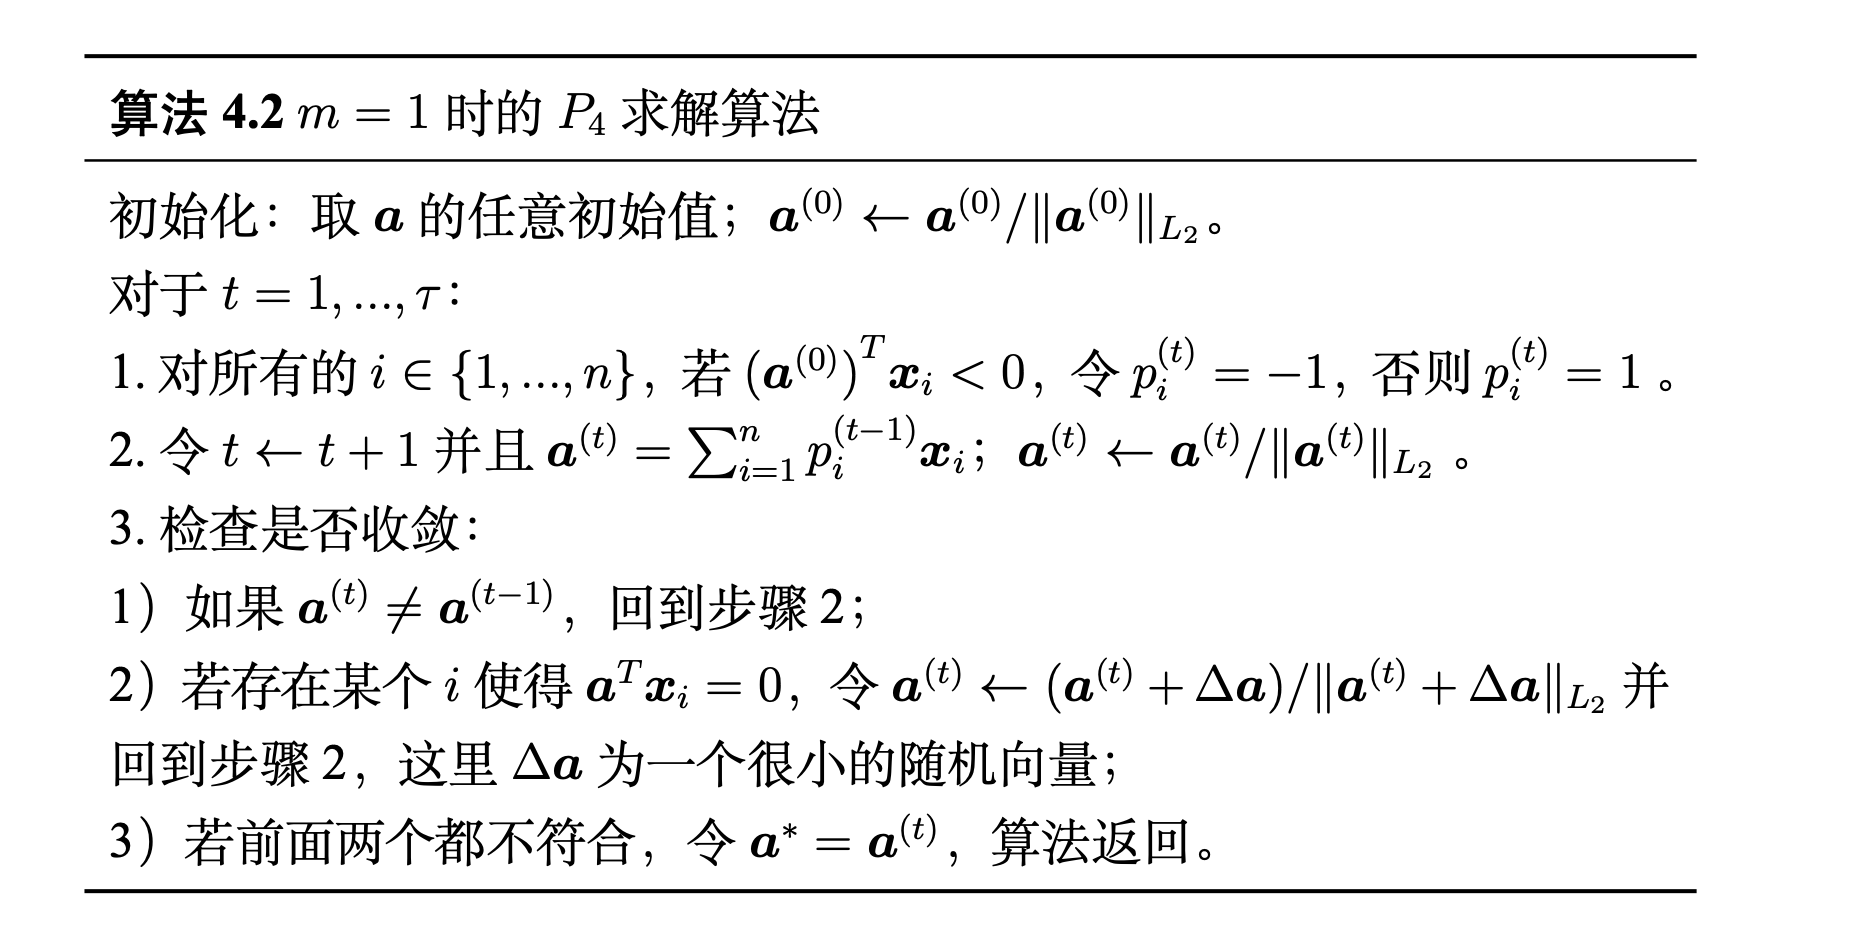
\includegraphics[width=10cm]{pics/kwak-1.png}
    \end{figure}
    \begin{itemize}
        \item 可以证明该算法在有限步骤内收敛到一个局部最优解。
    \end{itemize} 
\end{frame}

\begin{frame}{一种最大化特征空间投影$L_1$范数的贪婪算法}
    \begin{itemize}
        \item 利用贪婪策略,每次求解m为1的子问题,最终得出n个主成分。
    \end{itemize} 
    \begin{figure}
        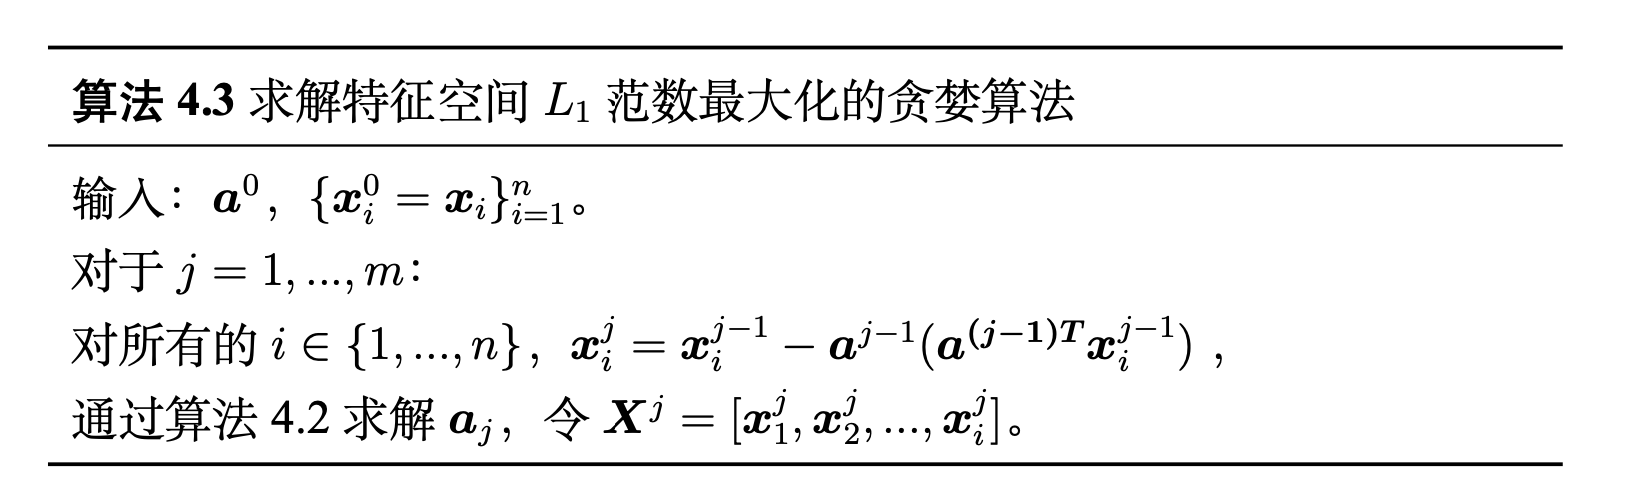
\includegraphics[width=10cm]{pics/kwak-2.png}
    \end{figure}
    \begin{itemize}
        \item 可以证明,算法中每次得到的主成分之间正交。
    \end{itemize} 
\end{frame}


\begin{frame}{数值模拟实验}
    \begin{itemize}
        \item 通过数值模拟实验,希望观察两种$L_1$主成分
        分析和$L_2$主成分析在稳健性和载荷矩阵上的对比。
        \item 可以发现,无论是哪一种$L_1$主成分分析都是
        对离群值稳健的。
    \end{itemize} 
    \begin{figure}
        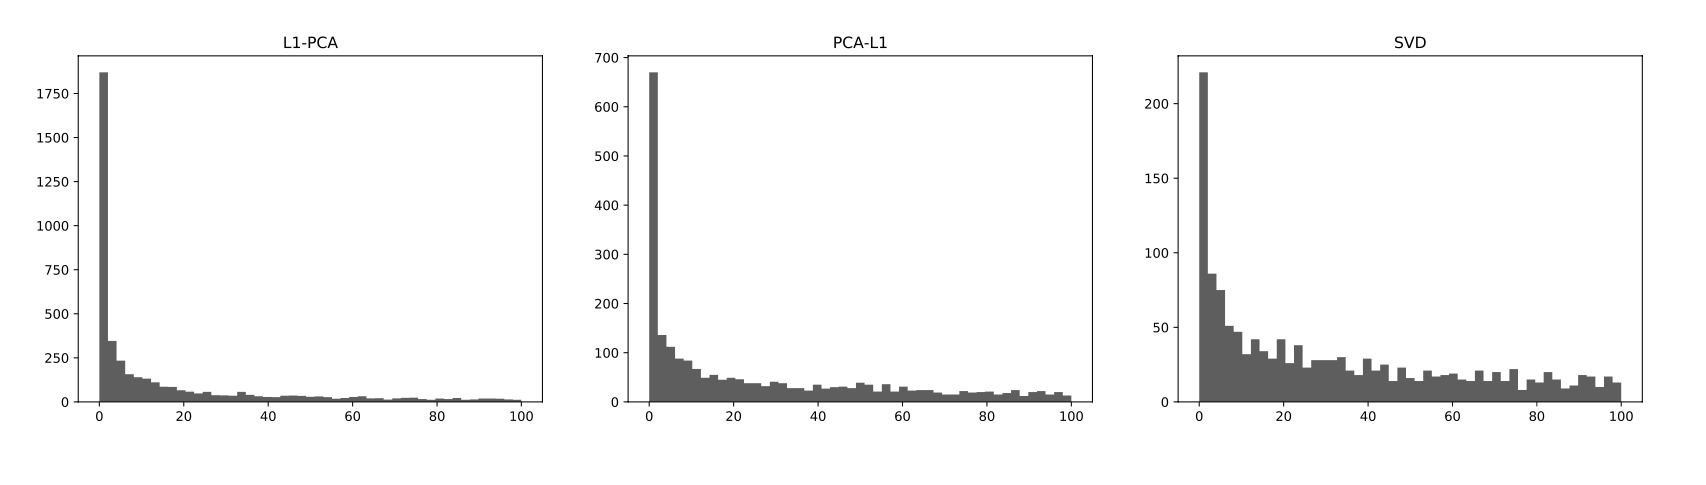
\includegraphics[width=10cm]{pics/compare-l1.png}
    \end{figure}

\end{frame}

\begin{frame}{数值模拟实验}
    \begin{itemize}
        \item 三种主成分分析得到的主成分是不同的。
        \item 将得到的因子载荷矩阵进行最大方差旋转,可更易看出区别。
    \end{itemize} 
    \begin{figure}
        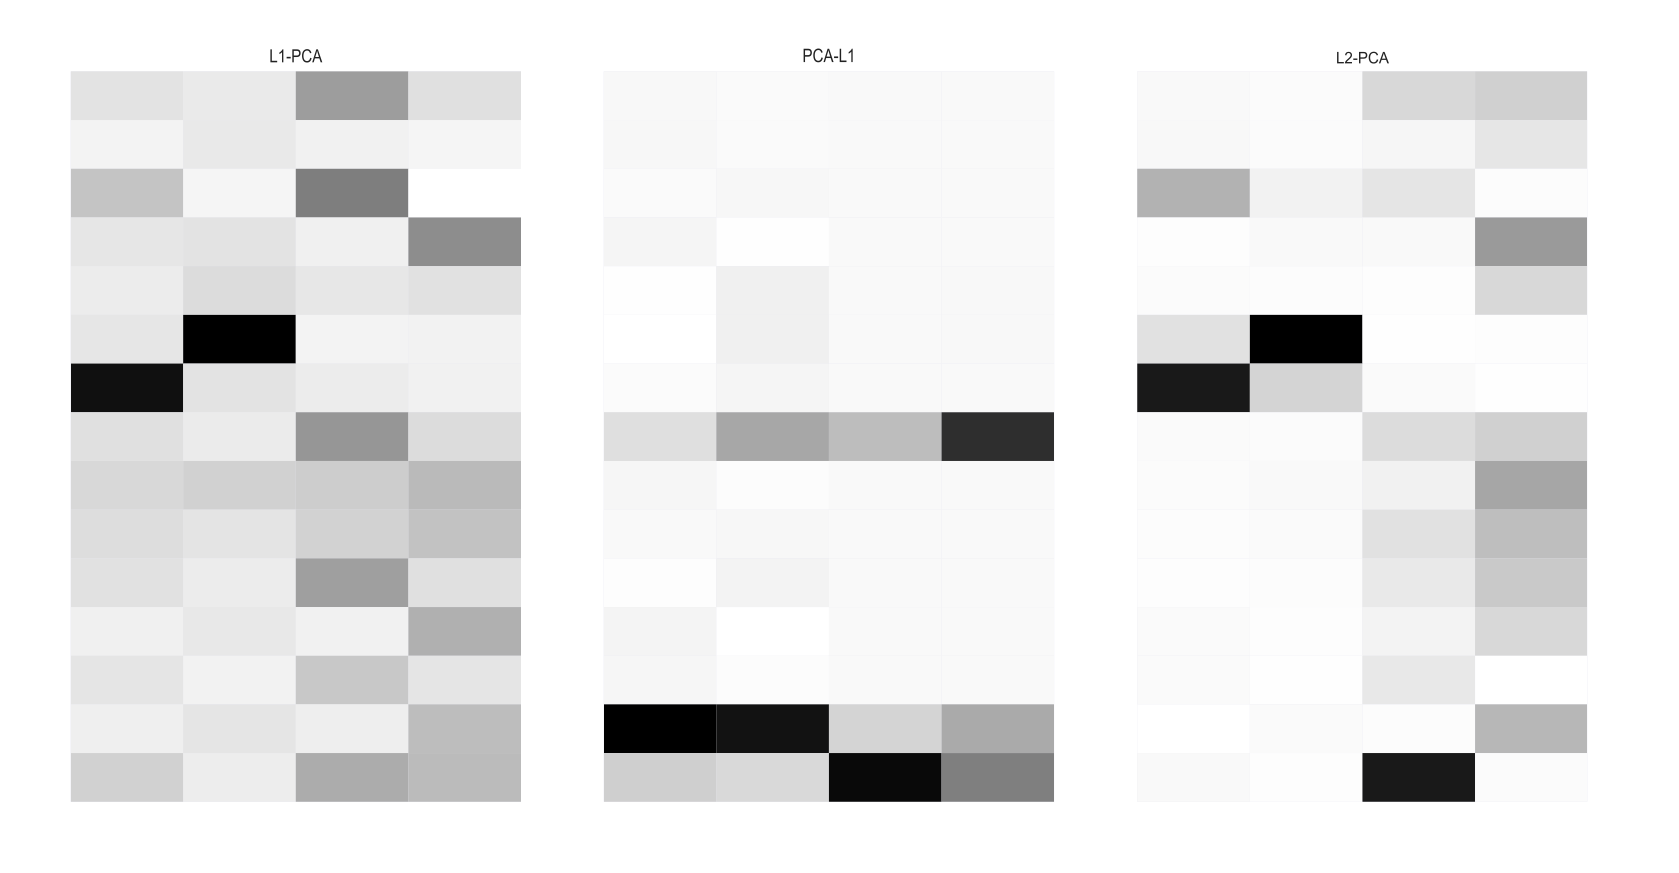
\includegraphics[width=10cm]{pics/loadings-compare.png}
    \end{figure}

\end{frame}


\begin{frame}{实证研究——扩散因子模型进行宏观经济预测}
    \begin{itemize}
        \item 将两种不同的$L_1$主成分分析都应用于扩散指数模型。
        \item 比较预测的准确性,结论是两种$L_1$因子都有良好的
        预测效果,均适用于稳健因子分析。
    \end{itemize} 

    \begin{table}[H]
        \centering
        \tiny
        \caption{向前一个月预测结果}
        \label{outcome4}
        \begin{tabularx}{\textwidth}{lXXXXXX}
        \toprule
                     &  MSE(L1 PCA) &  MSE(PCA L1) &  MAE(L1 PCA) &  MAE(PCA L1) &  MPAE(L1 PCA) &  MPAE(PCA L1) \\ \midrule
        消费者满意指数     & 0.81            & 0.78        & 0.87            & 0.83        & 0.43             & 0.67         \\
        工业生产者出厂价格指数 & 0.70            & 0.83        & 0.75            & 0.92       & 0.96             & 0.90         \\
        货币供应量M2      & 0.76            & 1.01        & 0.90            & 1.00       & 0.45             & 0.92         \\
        固定资产投资总额  & 0.89            & 1.11        & 0.97            & 1.03        & 0.81             & 1.05         \\
        房地产开发投资总额 & 0.79            & 0.94        & 0.95            & 0.97        & 0.91             & 1.10         \\
        社会消费品零售总额 & 0.84            & 0.62        & 0.87            & 0.78        & 0.45             & 0.76         \\
        制造业采购经理指数    & 1.24            & 0.99        & 1.06            & 1.14        & 0.90             & 0.82         \\
        住宅新开工面积总数  & 0.89            & 1.20        & 0.85            & 1.12        & 0.45             & 1.19         \\
        股票流通市值     & 0.99            & 1.23        & 0.98            & 1.12        & 0.81             & 0.98         \\
        消费者信心指数     & 0.93            & 0.70        & 0.98            & 0.80        & 0.98             & 0.99         \\ \bottomrule
        \end{tabularx}
    \end{table}
\end{frame}


\section{结束语}
\begin{frame}{注意}
    \begin{itemize}
        \item 本文所有实验均用Python编程实现了各算法伪代码。
        算法的计算性能与实现程序的质量关联很大,本文的运行时间
        仅做实验对比,不代表算法的标准性能。
    \end{itemize} 
    \small 以SVN算法的一次实现为例给出部分示例代码:
    \begin{figure}
        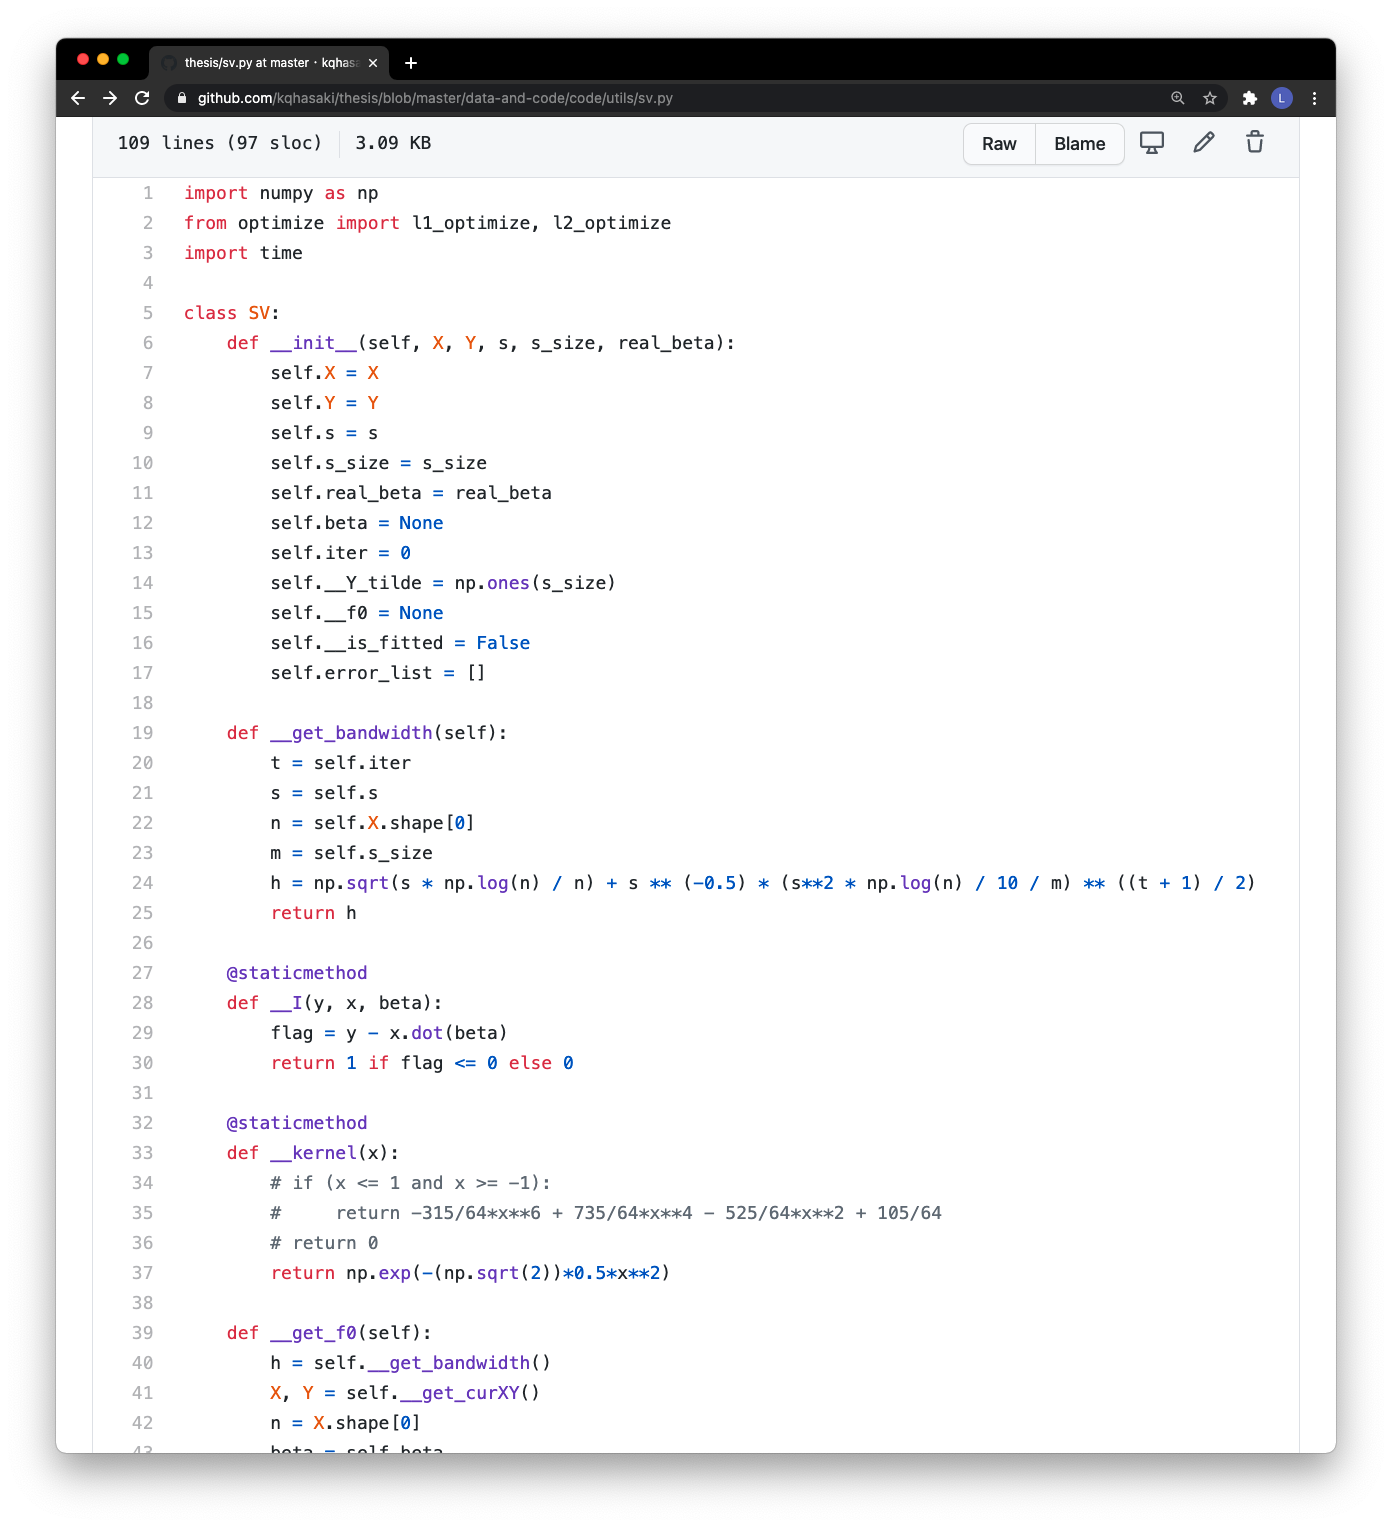
\includegraphics[width=7cm]{pics/code-demo2.png}
    \end{figure}

\end{frame}

\begin{frame}{注意}
    \begin{figure}
        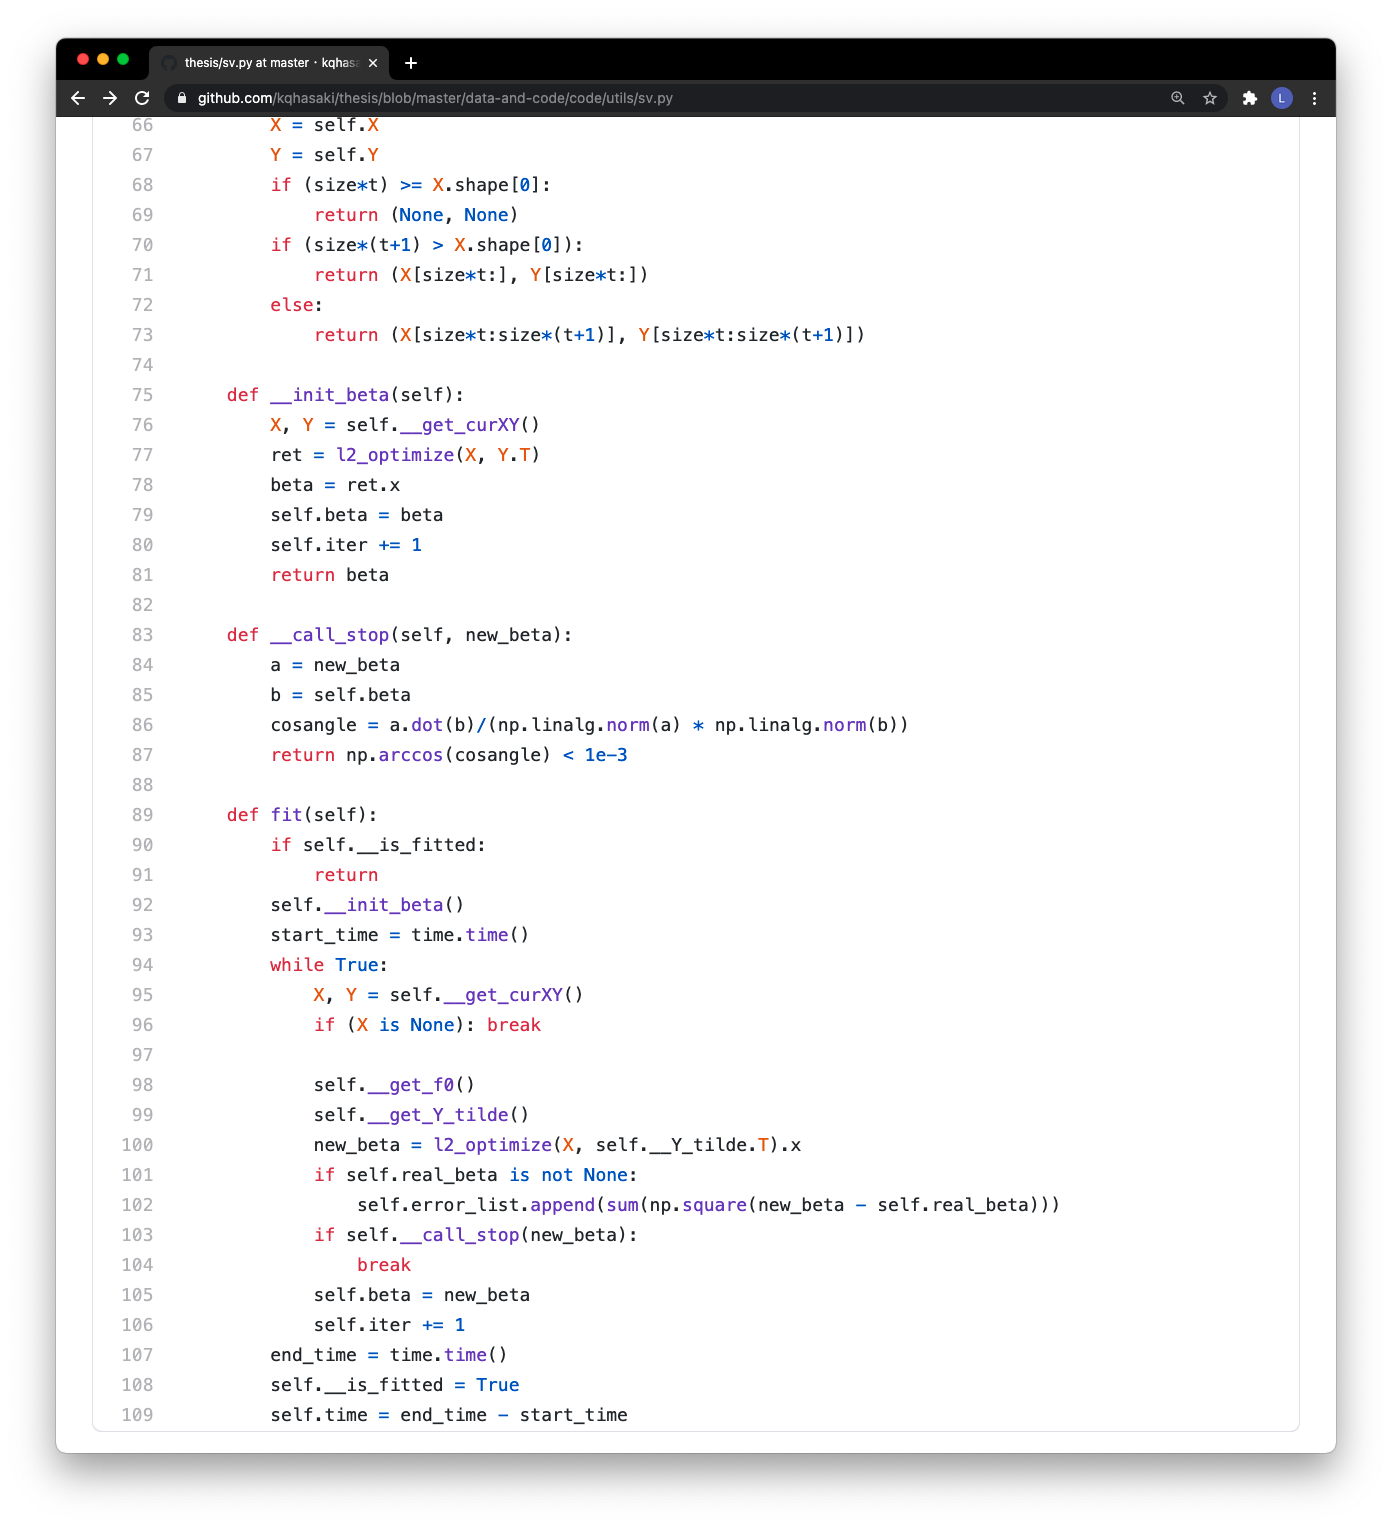
\includegraphics[width=7cm]{pics/code-demo.png}
    \end{figure}
\end{frame}

\begin{frame}{论文的创新点}
    \begin{itemize}
        \item 扩散指数模型进行经济预测时,使用$L_2$主成分估计因子;
        本文创新性地使用$L_1$主成分估计得到$L_1$因子,
        使得在处理重尾宏观经济数据时,预测更加准确、稳健性更好。
        \item 本文介绍并检验了两种最新的最小绝对值回归优化算法,
        并给出了使用建议。
        \item 利用最小绝对值回归优化算法,本文改进了经典的采用
        线性规划的交替凸优化算法,起到了一定的效率改进作用。
    \end{itemize}
\end{frame}



\begin{frame}{结束语}
    \centering
    \Large
    感谢到场的各位专家、教授、老师和同学!
\end{frame}
\end{document}
